\documentclass{article}
\usepackage{graphicx}
\usepackage{enumerate}
\usepackage{float}
\usepackage{amssymb, amsmath}
\usepackage{fancyvrb}
\usepackage{caption}
\usepackage{subcaption}
\usepackage[letterpaper, margin=1in]{geometry}


\begin{document}

\title{Assessment Report for AIA}
%\today
\author{KEE Consulting\\ 
        Los Angeles}

\maketitle
%\clearpage



\section{Data Infrastructure}

Overall the data infrastructure is in good shape. 
~\\
~\\
Greatest weakness of current dataset is that it is being populated by numerous agents each with varying standards.  This poses two problems:

\begin{itemize}
\item The accuracy of the data becomes questionable:

A bond with a ``discharged'' status may or may not have been forfeited. This makes the use of the bond status unreliable by itself.  
 
\item The variability of the data becomes unmanageable:

For data analysis to work, non-numerical data must be categorized. This allows the mathematical models to translate each category to numeric form (i.e. Male/Female $\rightarrow$ 0/1), currently:  
\begin{itemize}
\item Charges associated with bonds are filled with either state-dependent criminal codes, abbreviated crime, generalizations, or left blank altogether. A suggestion would be to have drop down menu with a severity rank of crime.  
\item Defendant employment information is often filled with a business name or ``self employed'', which by itself is not very useful. A useful substitute could be an income bracket information from a drop down menu. 
\item Defendant relationships are filled with strings such as ``babby mama''. Solution would be to provide options (i.e. ex-partner).
\end{itemize}
\end{itemize}
~\\
\section{Project Road-maps}

\subsection{Project A : \underline{A logistic regression model for Failure to Appear}}
\subsubsection{The Goal}
The goal is to construct a model which relates the probability of failure to appear (FTA) to variables through a coefficient for each variable. The Vision dataset is used jointly with the AIMS dataset. 
~\\
~\\
A regression model: A statistical analysis used to predict scores on an outcome
variable based on scores on one or more predictor variables.\\
~\\
Can be as simple as:
\begin{equation}
Y = B_{0} + B_{1}X_{1} + B_{2}X_{2} + \ldots + \epsilon_{1}+\epsilon_{2} + \ldots \\
\end{equation}
\begin{itemize}
\item Y: outcome variable (ex: Will fail to appear?)
\item X: predictor variables (ex: Defendant's age, bail amount \ldots)
\item B: coefficients relating X's and Y
\item $\epsilon$: error terms (a.k.a residual)
\end{itemize}
~\\


\subsubsection{Validity of model}

As a proof of concept, four data variables were looked at for the initial model: \\
~\\
\textbf{Characteristic of the defendant:}
~\\ 
\begin{enumerate}
\item Age at time of the bond
\begin{figure}[H]
\centering
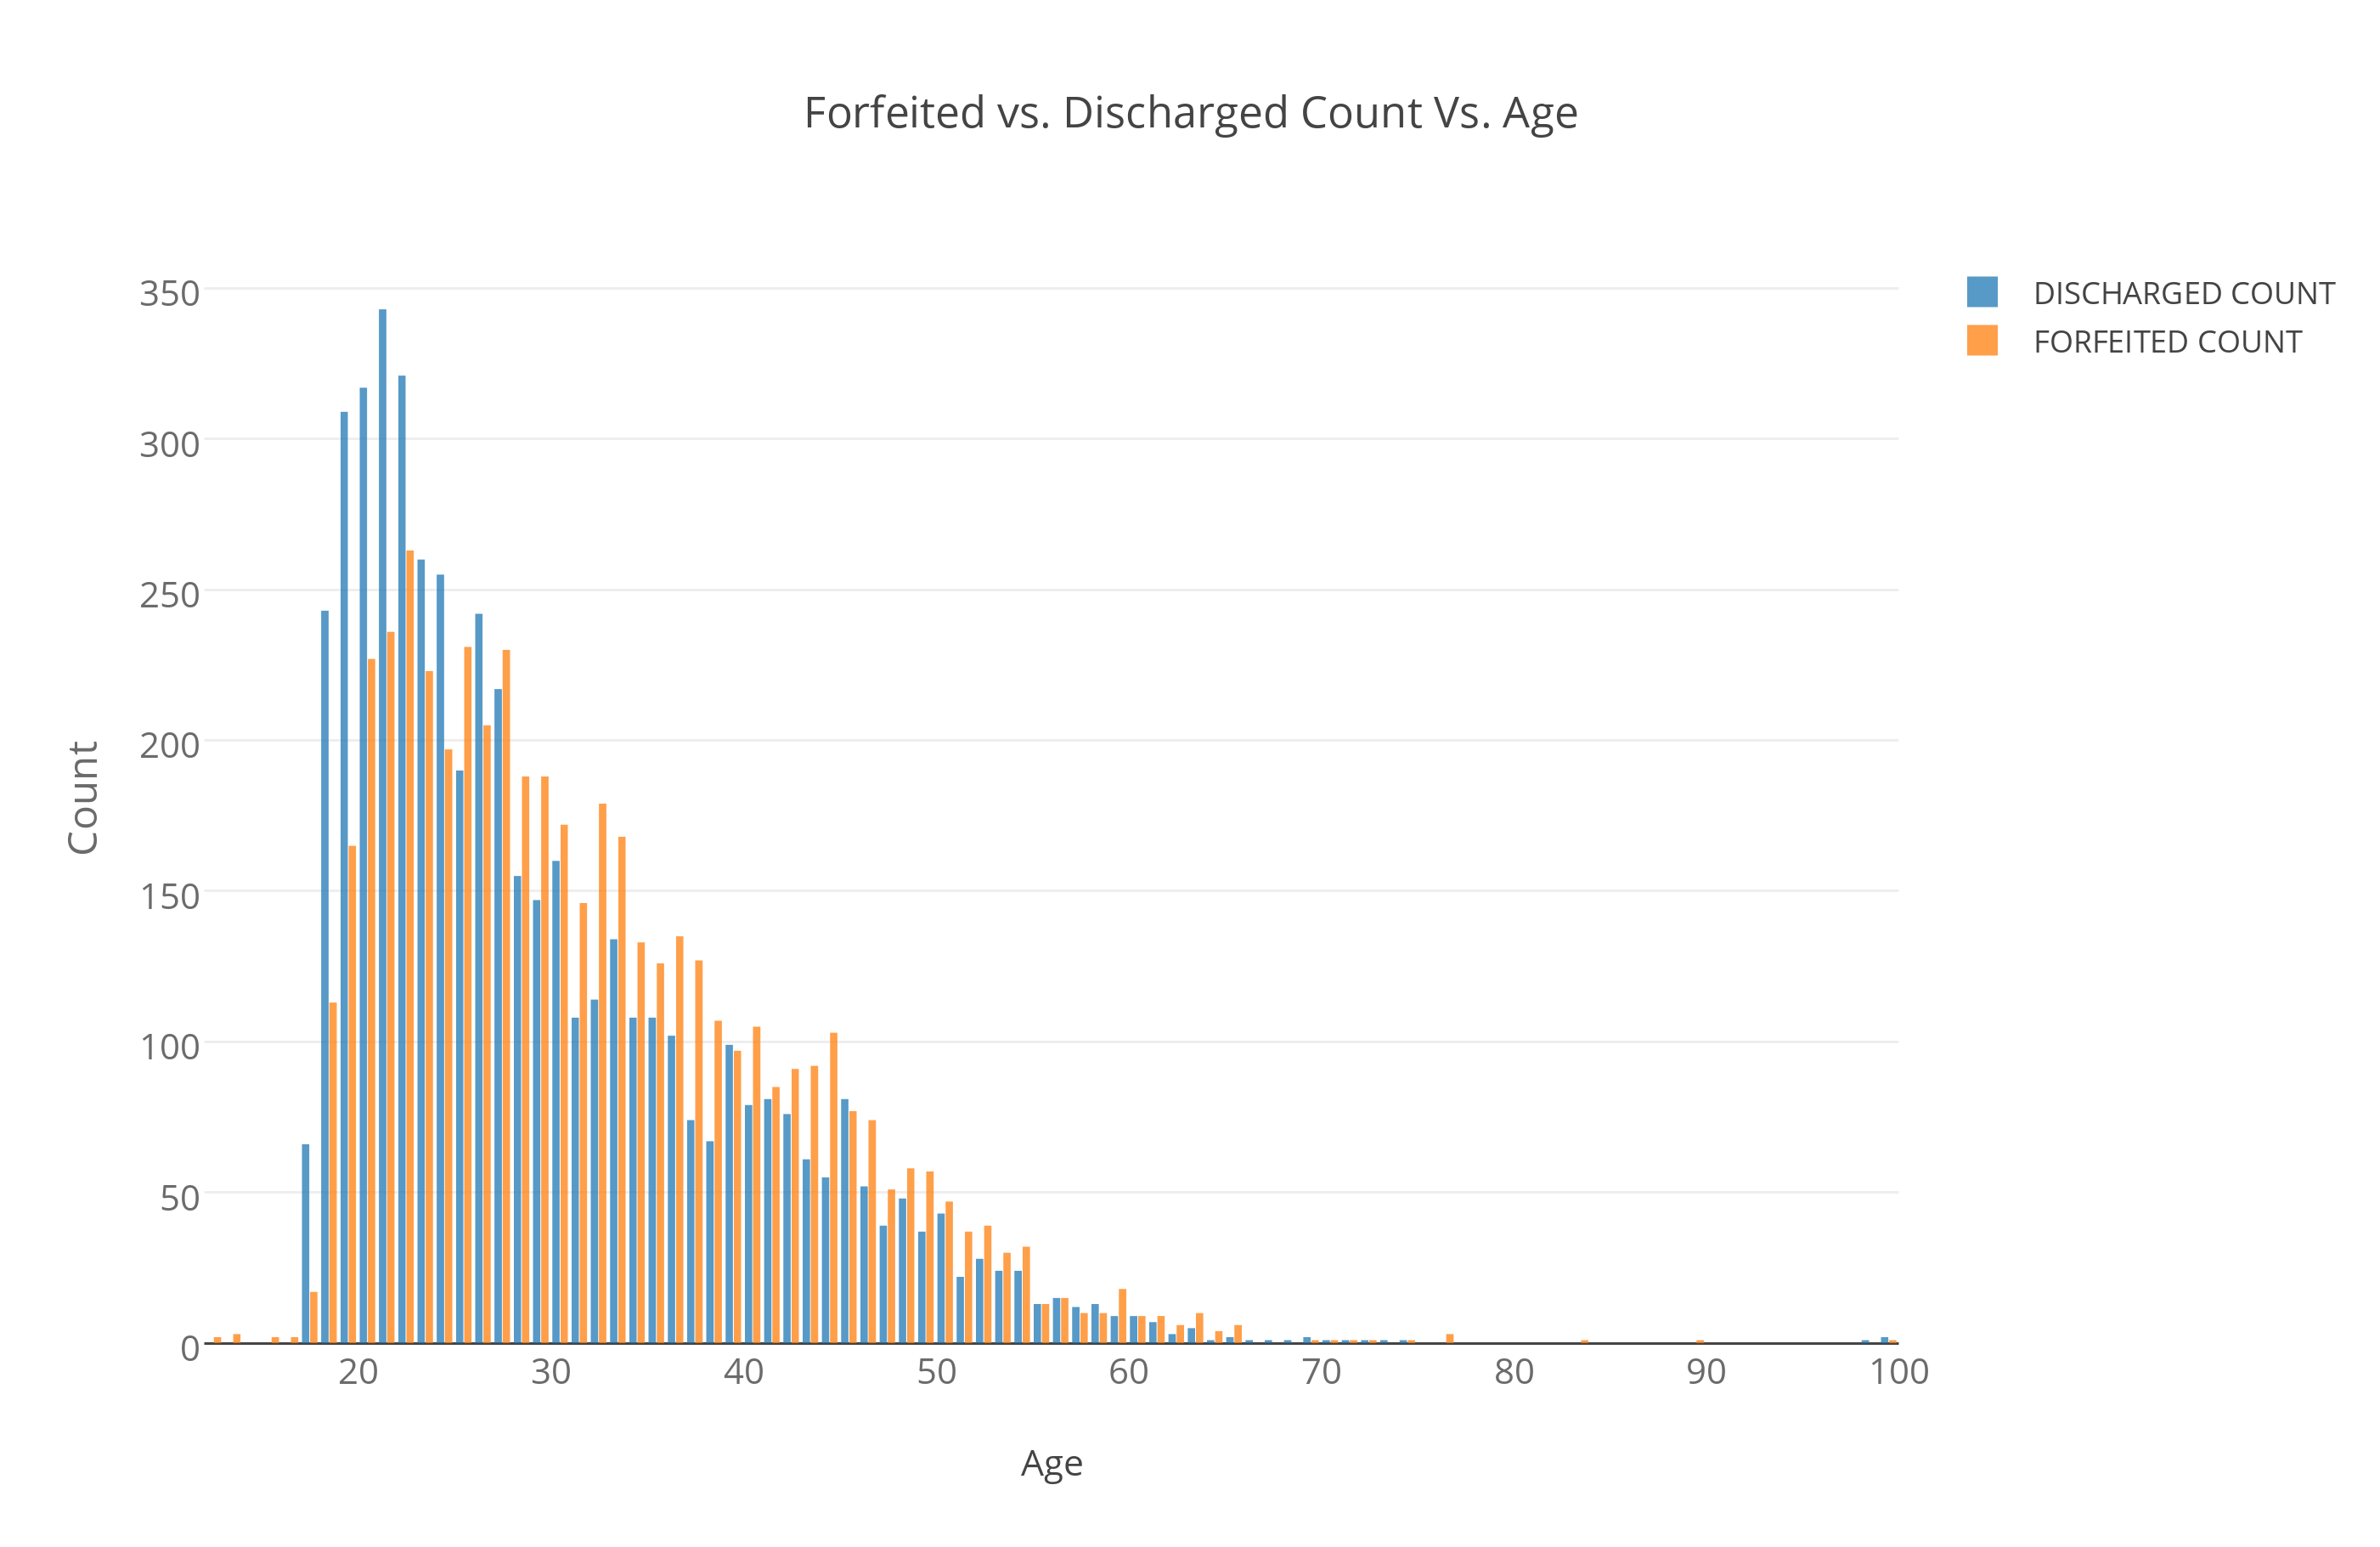
\includegraphics[width=0.5\paperwidth]{Forfeited_vs_Discharged_Count_Vs_Age.png}
\end{figure}

\item Gender
\begin{figure}[H]
\centering
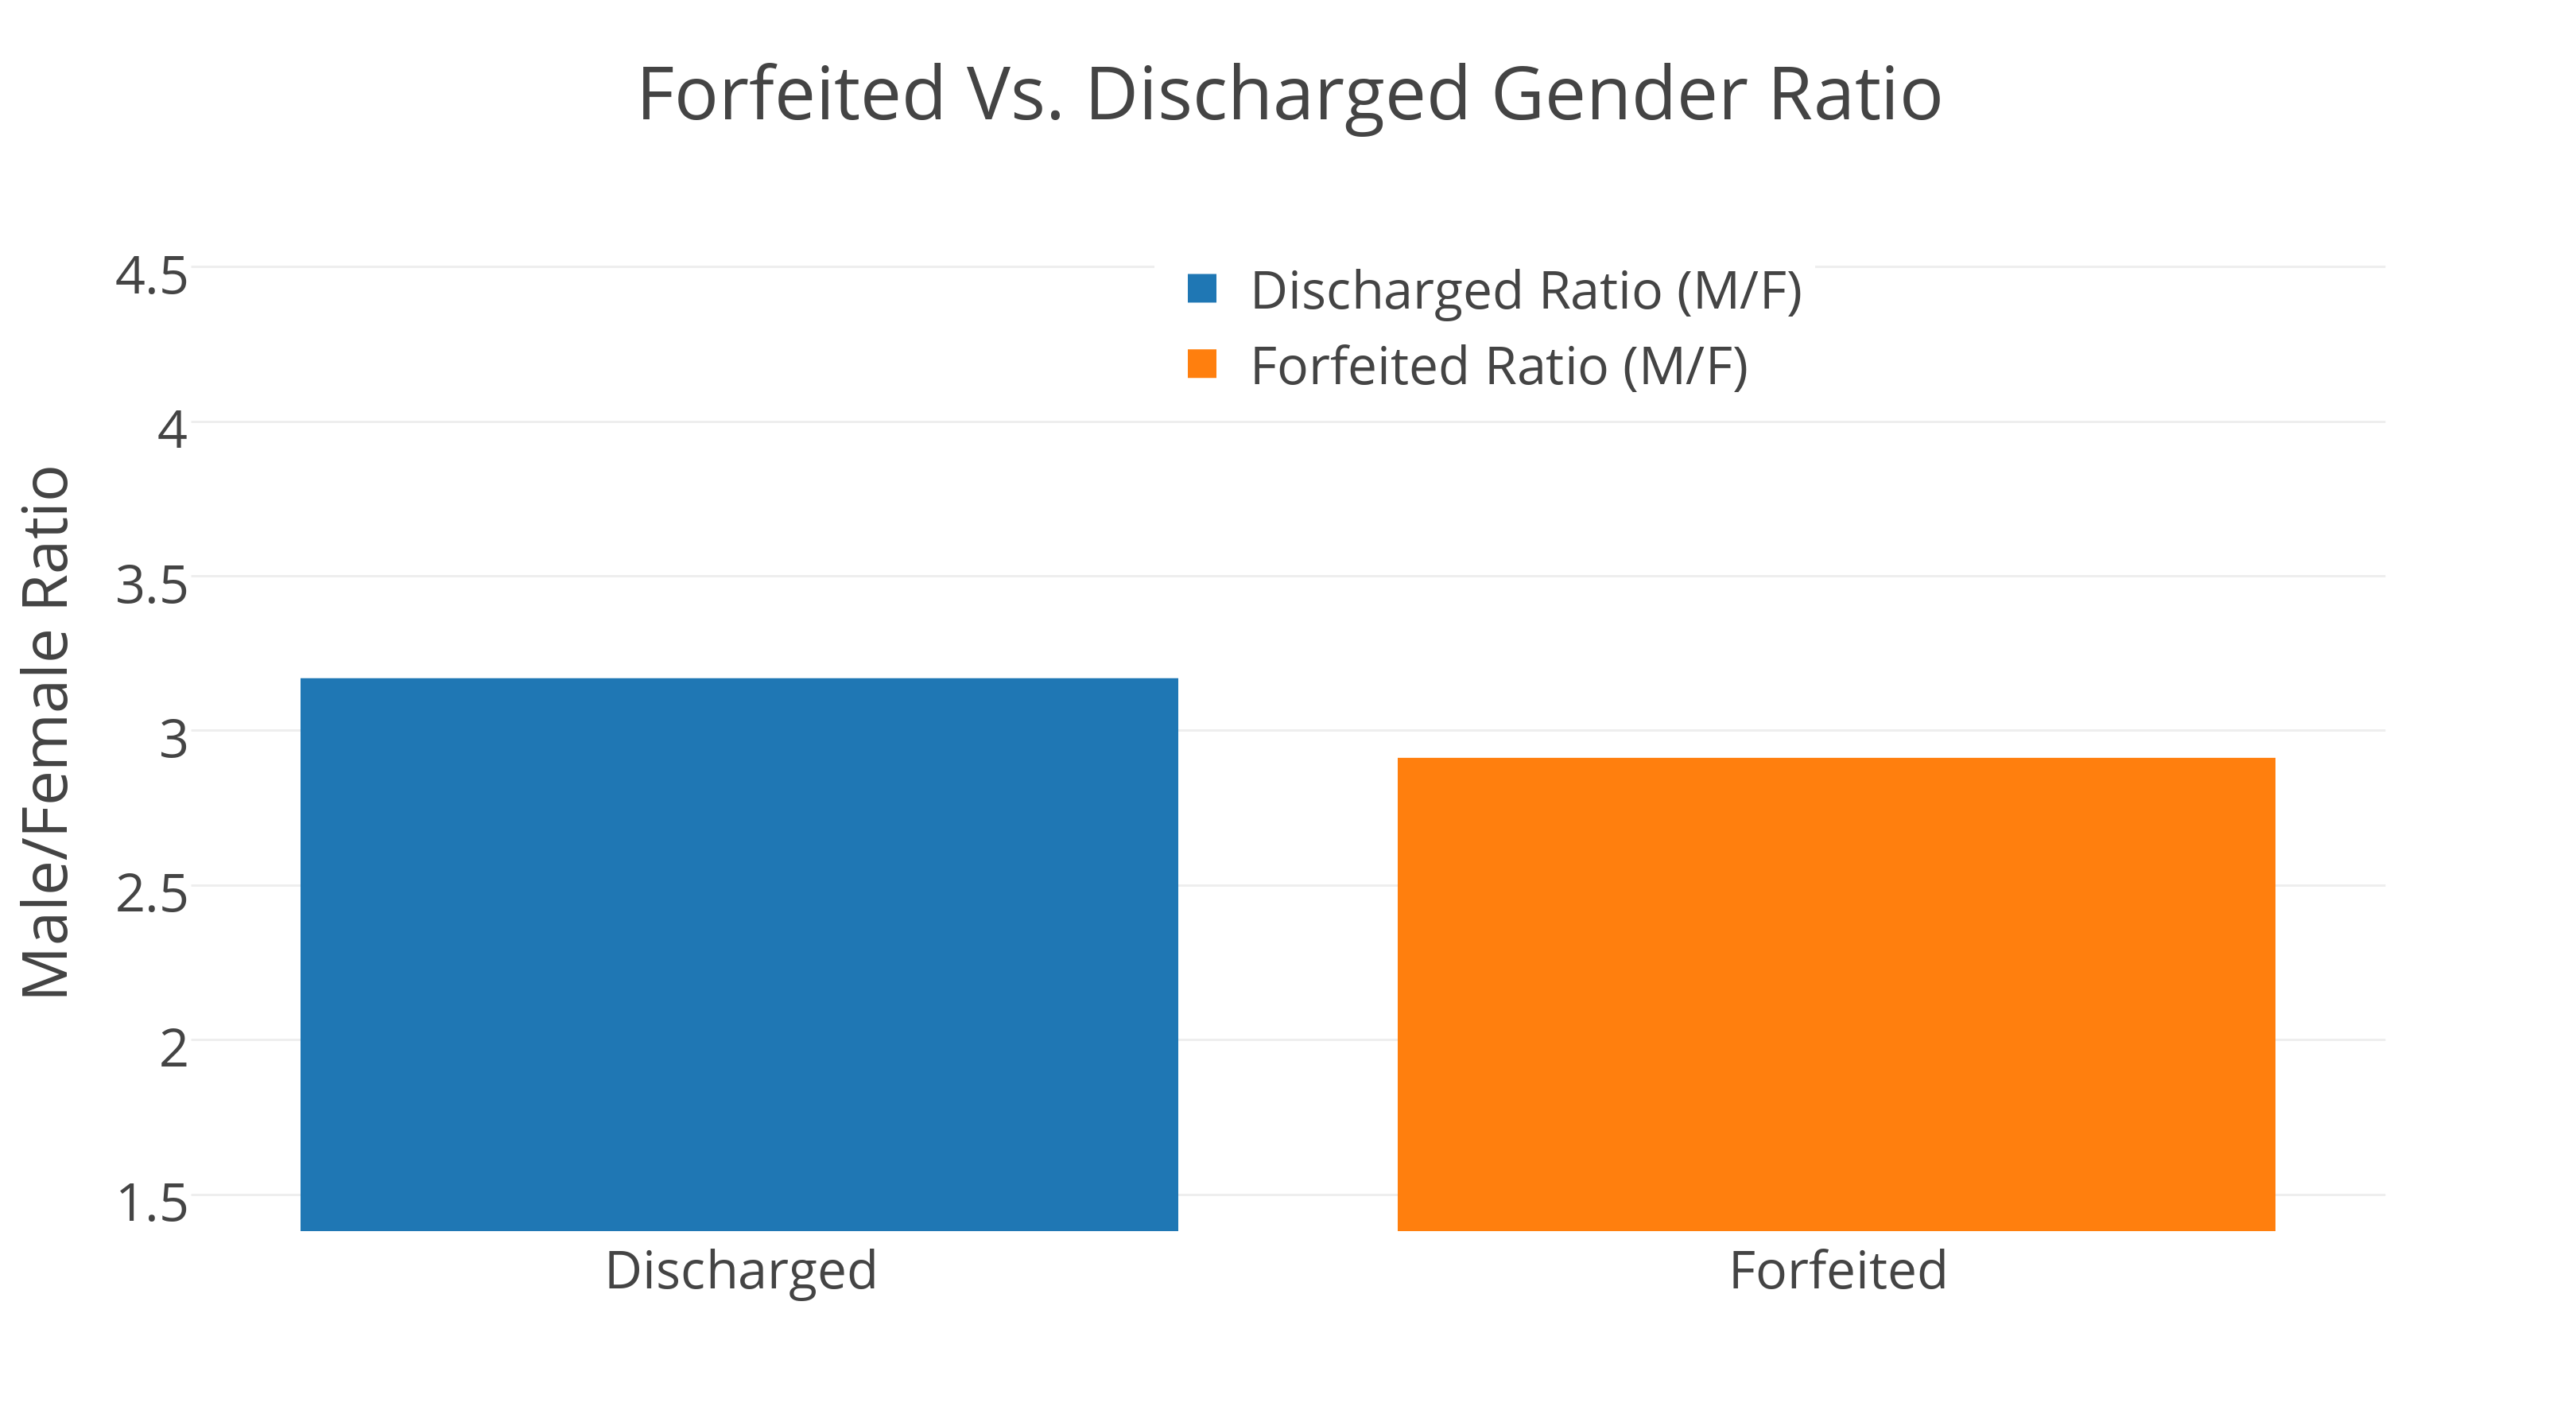
\includegraphics[width=0.5\paperwidth]{Forfeited_vs_Discharged_Gender.png}
\end{figure}

\end{enumerate}
~\\
\textbf{Characteristic of the environment:}
~\\
\begin{enumerate}
\setcounter{enumi}{2}
\item zipcode $\rightarrow$ income
\begin{figure}[H]
\centering
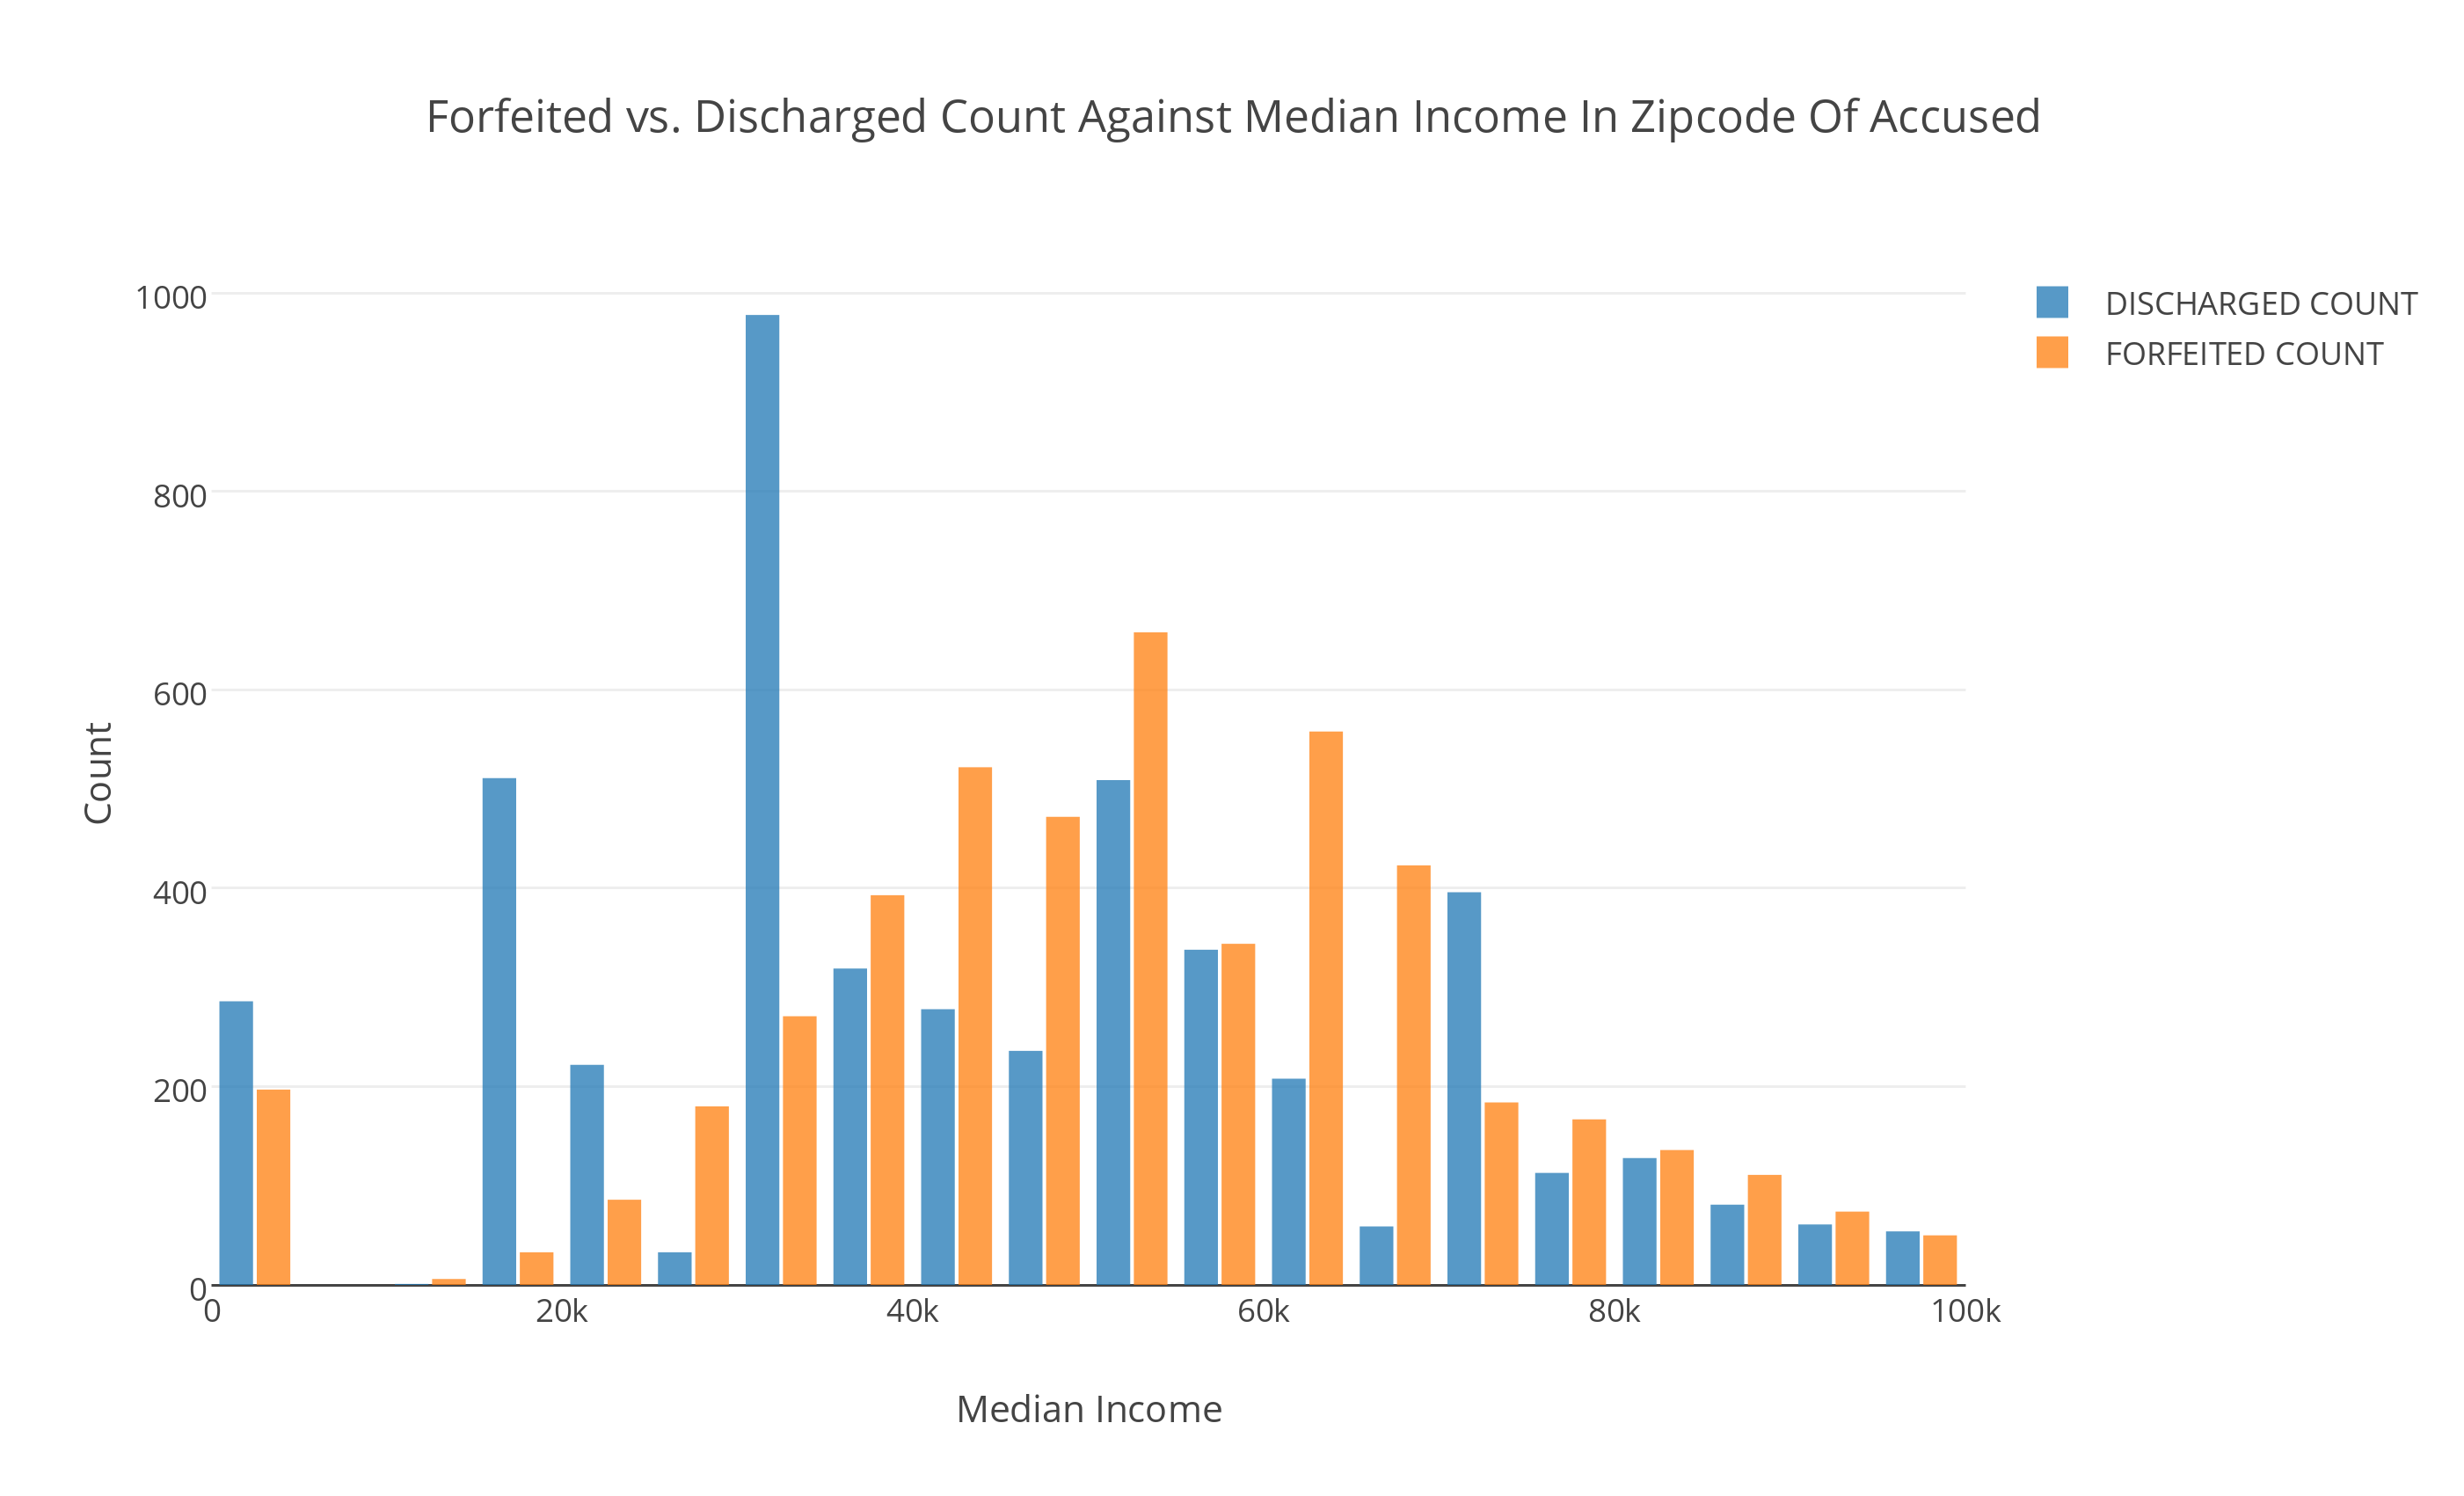
\includegraphics[width=0.5\paperwidth]{Forfeited_vs_Discharged_Count_Against_Median_Income_In_Zipcode_Of_Accused.png}
\end{figure}

The average income for a zipcode was obtained through an api to the latest available U.S. Census.   
\end{enumerate}
\textbf{Characteristic of the bond:}
~\\
\begin{enumerate}
\setcounter{enumi}{3}
\item Bond Amount
\begin{figure}[H]
\centering
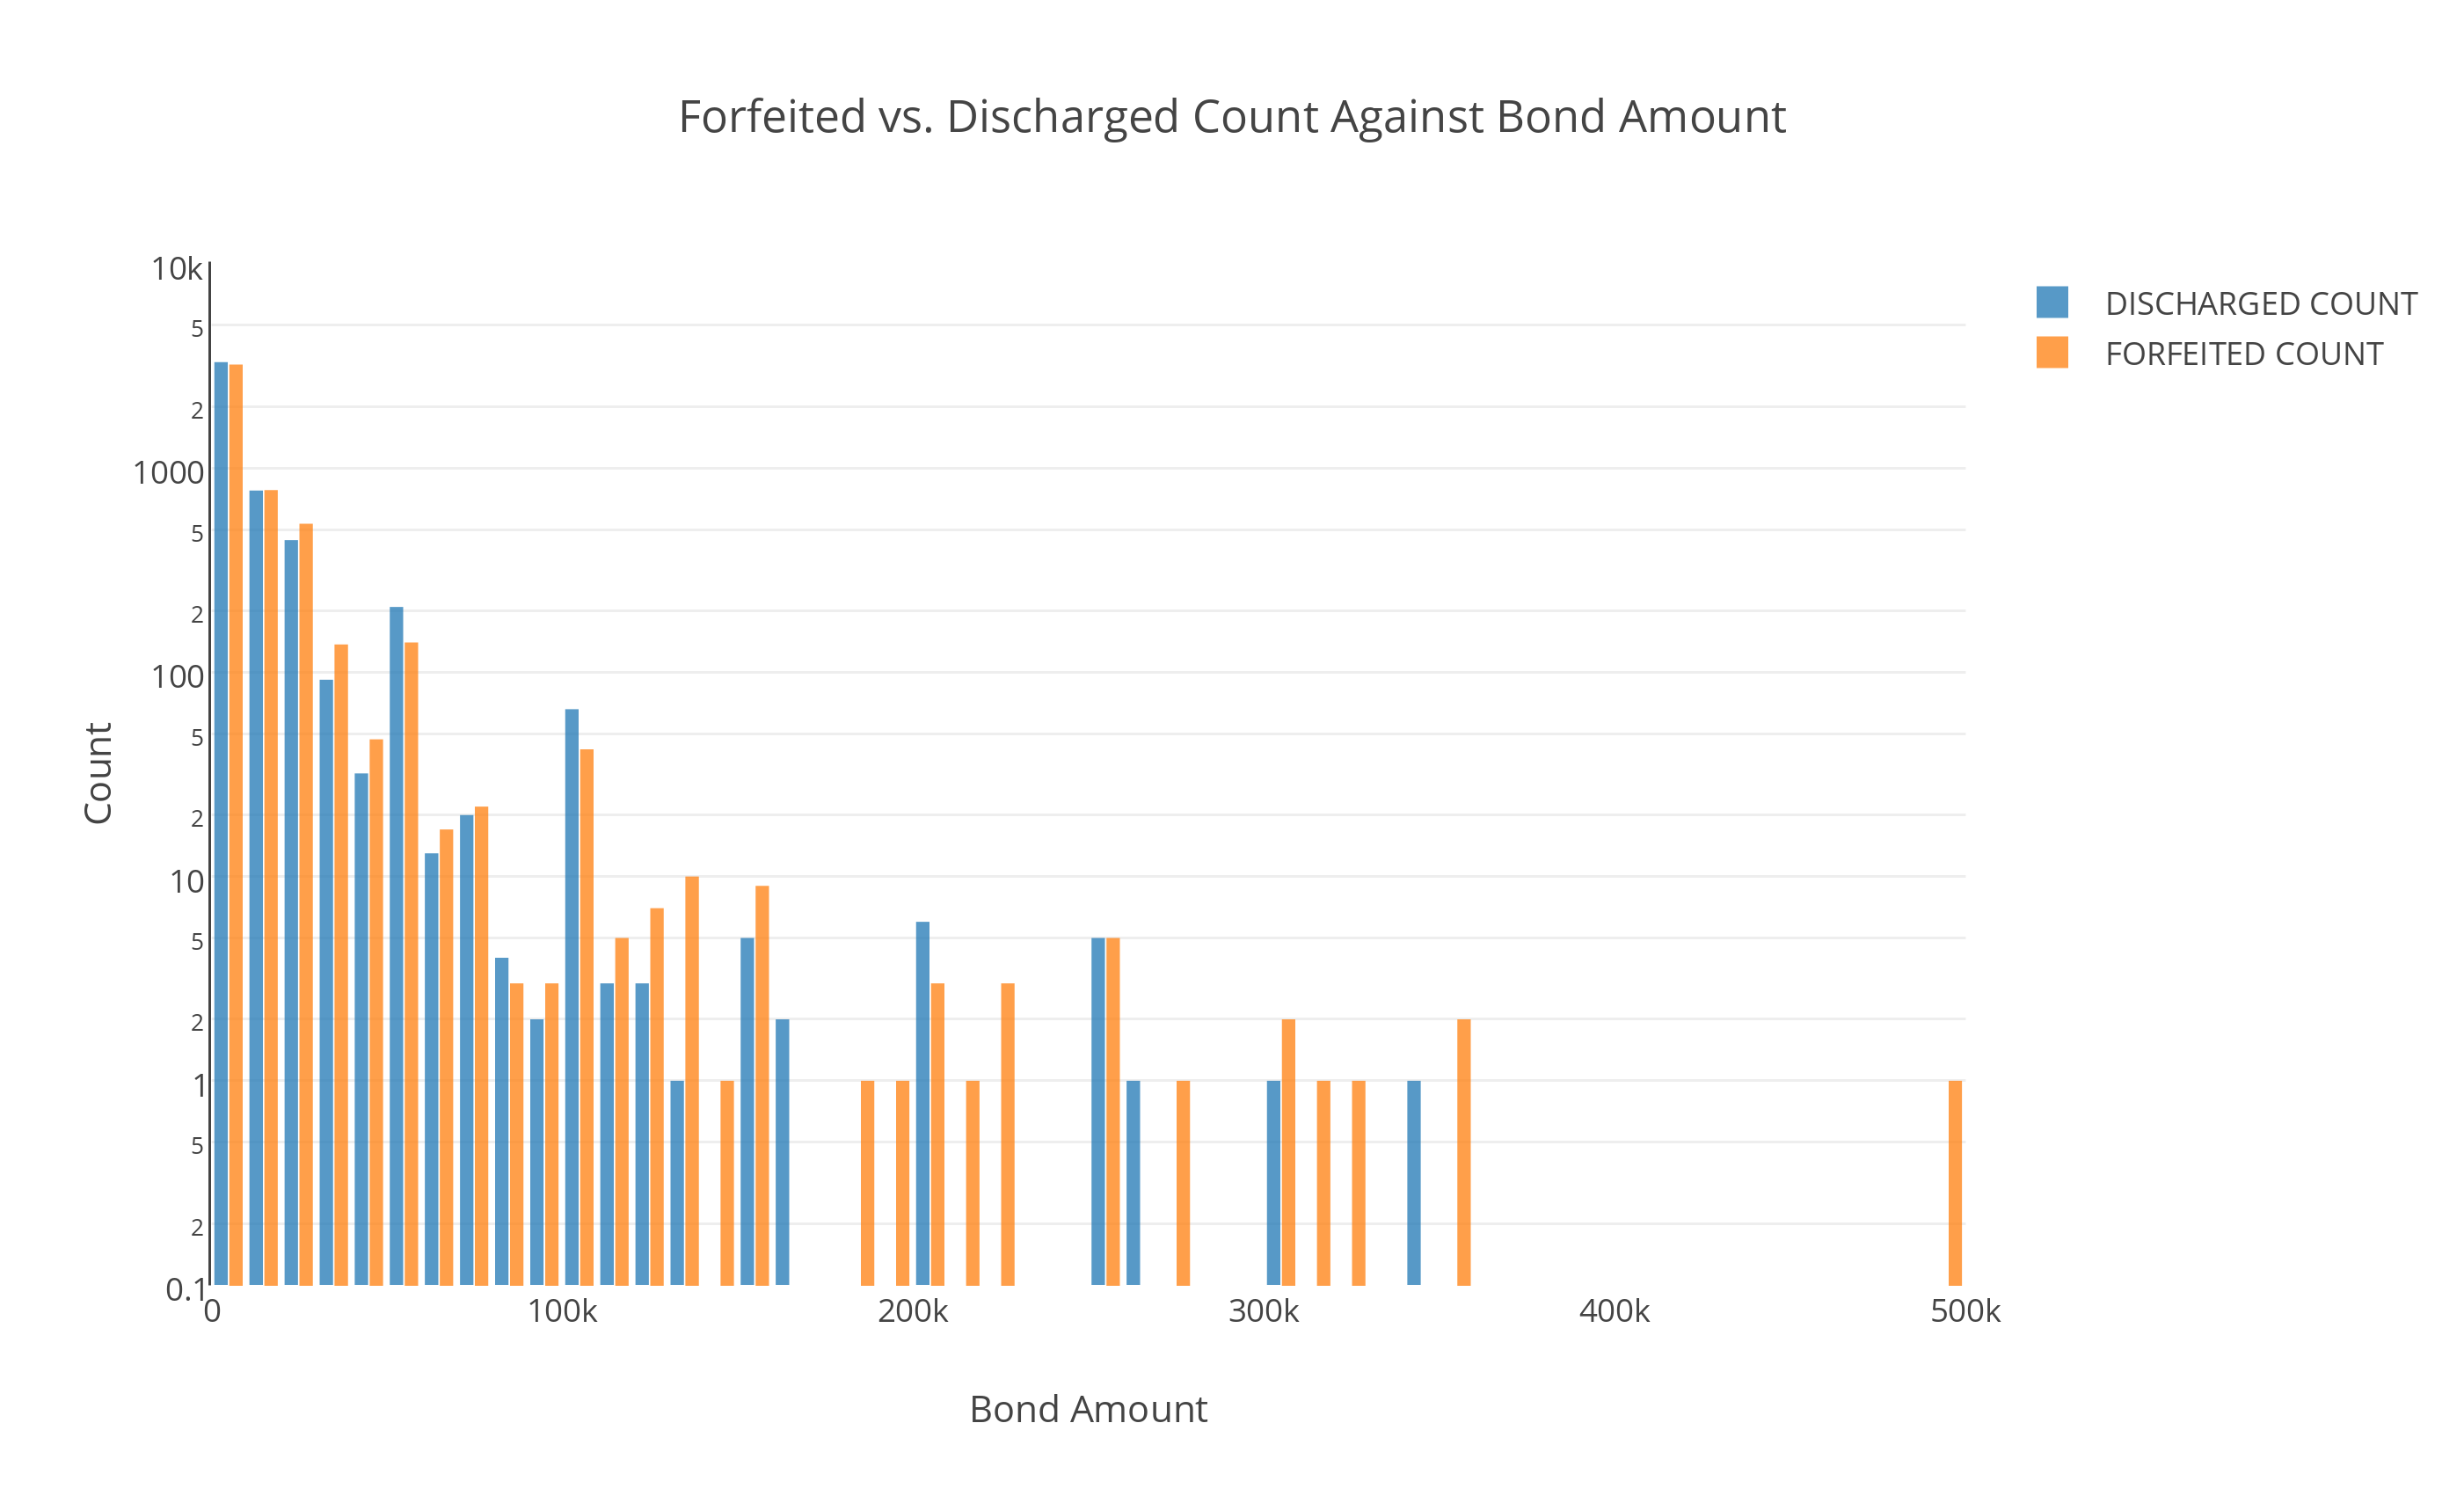
\includegraphics[width=0.5\paperwidth]{Forfeited_vs_Discharged_Count_Against_Bond_Amount.png}
\end{figure}
\end{enumerate}
~\\
\textbf{Running the Model:}
~\\
Finding a relationship between X and Y which minimizes the model errors gives us:


\begin{figure}[H]
\centering
\begin{BVerbatim}
Deviance Residuals: 
    Min       1Q   Median       3Q      Max  
-2.3472  -1.0933  -0.7349   1.1296   1.8166  

Coefficients:
                Estimate Std. Error z value Pr(>|z|)    
(Intercept)    -1.835339   0.099919 -18.368  < 2e-16 ***
catBond_Amount  0.013388   0.006470   2.069  0.03854 *  
age             0.031466   0.002381  13.213  < 2e-16 ***
catZipIncome    0.183926   0.010761  17.092  < 2e-16 ***
genderM        -0.166691   0.053297  -3.128  0.00176 ** 
---
Signif. codes:  0 ‘***’ 0.001 ‘**’ 0.01 ‘*’ 0.05 ‘.’ 0.1 ‘ ’ 1
\end{BVerbatim}
\end{figure}

%\begin{tabular}{ l | c | c }
%Variables & Defendant 1 & Defendant 2 \\
%\hline
%Age & 38  & 23 \\
%\hline
%Gender & Female & Male \\ 
%\hline
%Bond Amount & \$35,000 & \$5,000 \\ 
%\hline
%Zipcode Income & \$75,392 & \$101,905 \\
%\hline
%\hline
%calculated probablity of FTA & 75\% & 62\% \\
%& True Positve & False Positive
%\end{tabular}
%
~\\
example model predictions:
~\\
~\\
\underline{Defendant 1:}
~\\
\begin{itemize}
\item Age: 38
\item Gender: Female 
\item Bond Amount \$35,000
\item Zipcode Income  \$75,392
\item Known to have failed to appeared
\end{itemize}
~\\
Probability calculated by the model: 75\% to fail to appear
In reality, the bond was forfeited. This is called a ``true positive''.


~\\
\underline{Defendant 2:}
~\\
\begin{itemize}
\item Age:             23   
\item Gender:          Male
\item Bond Amount:    \$5,000
\item Zipcode Income: \$101,905
\item Known to have appeared
\end{itemize}
~\\
Probability calculated by the model: 62\% to fail to appear
In reality, the defendant appeared in court and the bond was discharged. 
This is called a ``false positive''.
~\\
~\\
The aim is to maximize true positives and minimize false positives. 


\begin{figure}[H]
\centering
%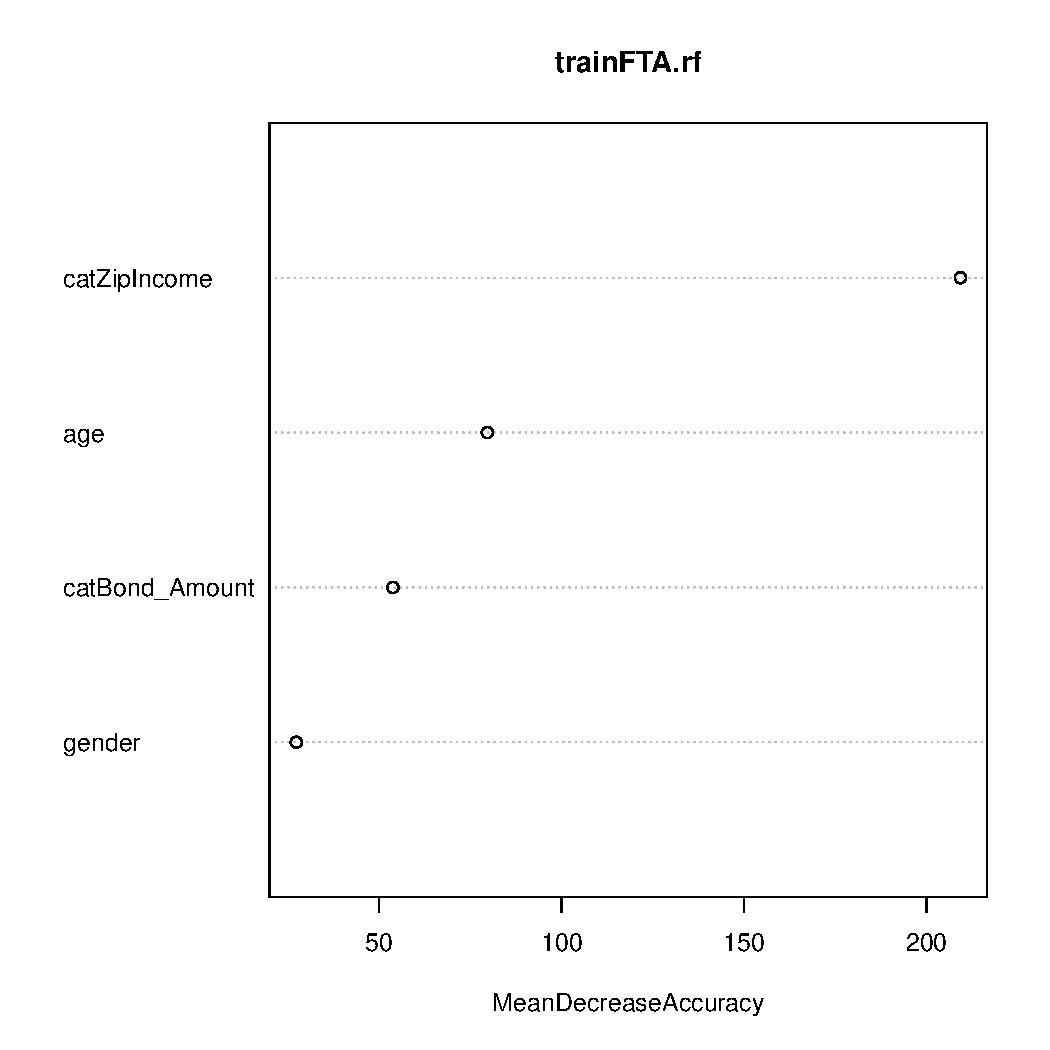
\includegraphics[width=0.45\paperwidth,page=1]{varPlot.pdf}
\includegraphics[width=0.40\paperwidth,page=3]{varPlot.pdf}
\end{figure}
 
\subsubsection{Deliverables and Work Estimate}
A ``model'' (equation) which would allow an agent to calculate the probability of FTA given the characteristics of the defendant and the bond.
The validity and performance of the model will be fully tested and reported. 
~\\
~\\
\textbf{1 month at \$80/hour = \$12,800}

\clearpage
\subsection{Project B: \underline{Agent Performance}}
~\\
\subsubsection{Ranking}
Ranking system: \textit{Going beyond total premium brought in:} \\
~\\
Goal: Construct an agent ranking system to assess the ``health'' of an 
agent's business. The metric should be intelligent enough to fairly compare agencies nationwide. 
For example it cannot focus solely on the total penal written, as this unfairly compares 
agencies in areas of differing crime rates. The ranking metric should be built robust 
against monthly fluctuations in penal written (for example a trend analysis can be incorporated.)


\subsubsection{The Arising Question}

We believe that after establishing the ranking, a primary question will arise that we propose to answer 
in this project. It is hard to predict what that question will be, but we work through an example below.  
%For example 
%an agent with a low penal but good ``health'' could indicate a bottlneck in the business. Is the agent too 
%conservative? Or is the premium rate too high? The underwriting limit too low? Etc...

~\\
~\\
\underline{Example Question:}
\begin{center}
\begin{quote}
\textit{What contract variables contribute to premium collected? Is it Premium Rate? BUF Rate? Underwriting limit? Others?}
\end{quote}
\end{center}

~\\
Testing ``Premium Rate'':
~\\
~\\
The following figures show the premium collected from agents throughout their numerous contracts with AIA:

\begin{figure}[H]
\begin{center}
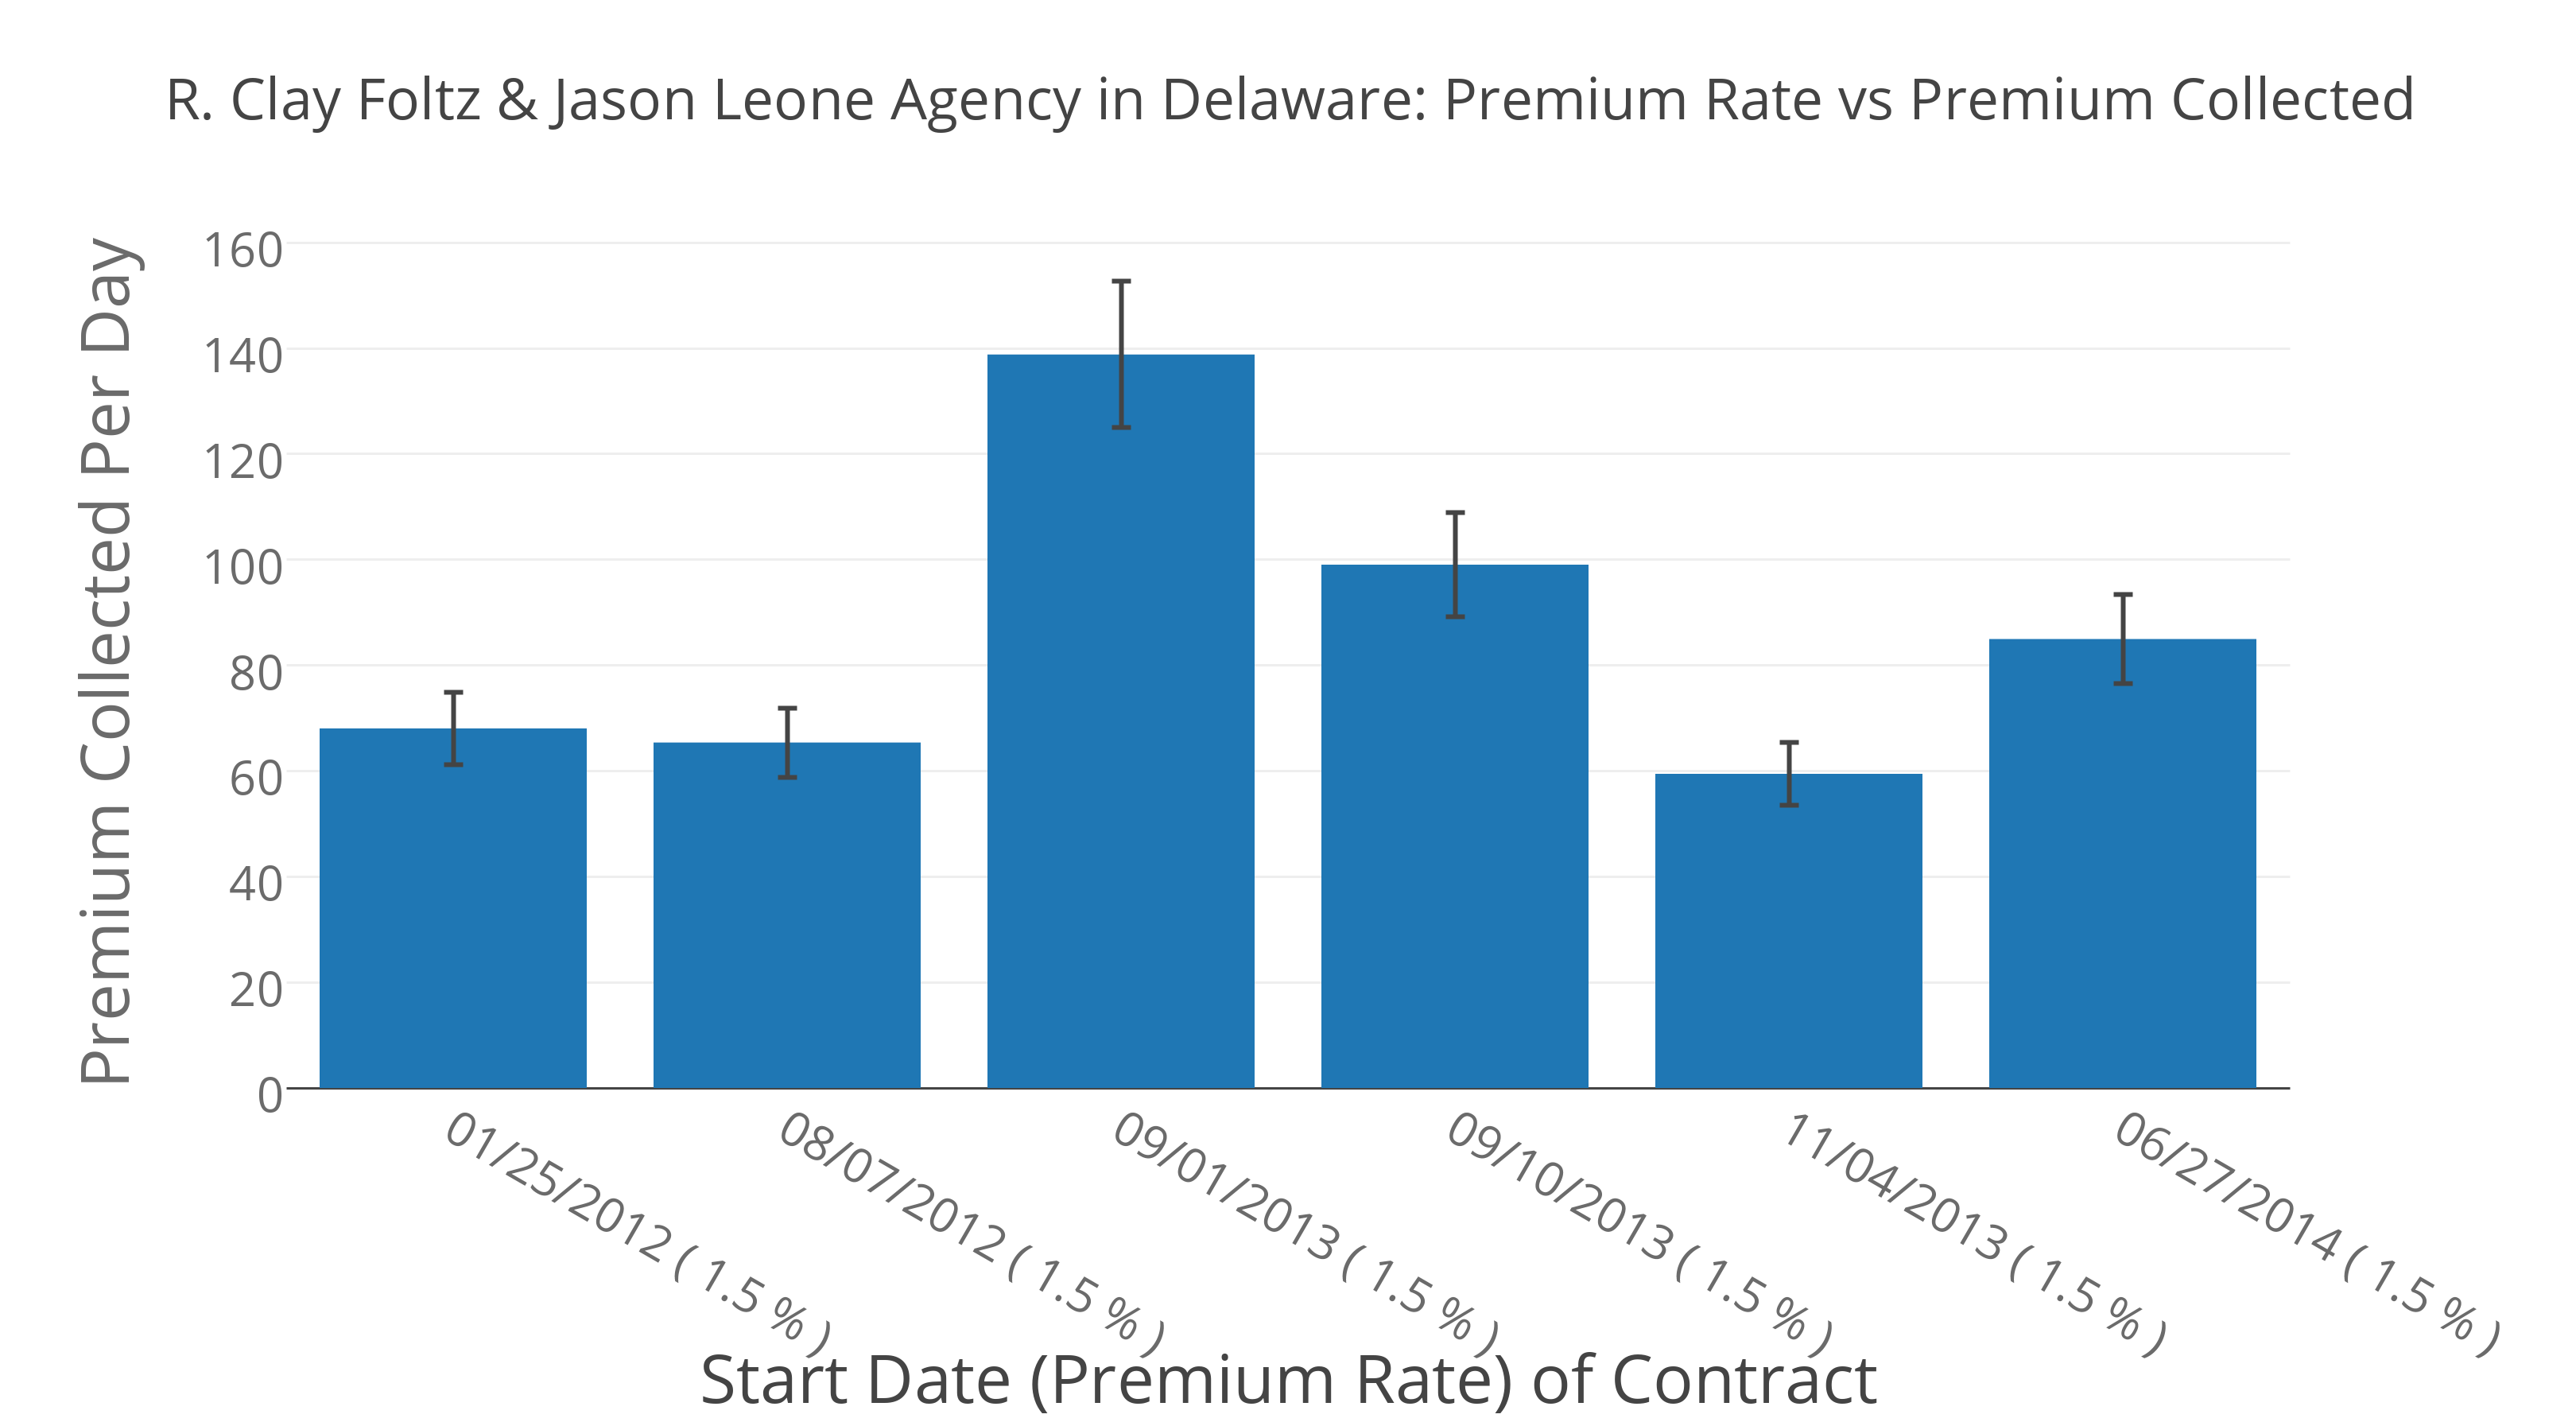
\includegraphics[width=.5\textwidth]{R_Clay_Foltz_&_Jason_Leone_Agency_in_Delaware-_Premium_Rate_vs_Premium_Collected.png}\\
\caption{An agent with a constant premium rate}
\end{center}
\end{figure}

\begin{center}
\begin{figure}[H]
\begin{subfigure}[b]{0.5\textwidth}
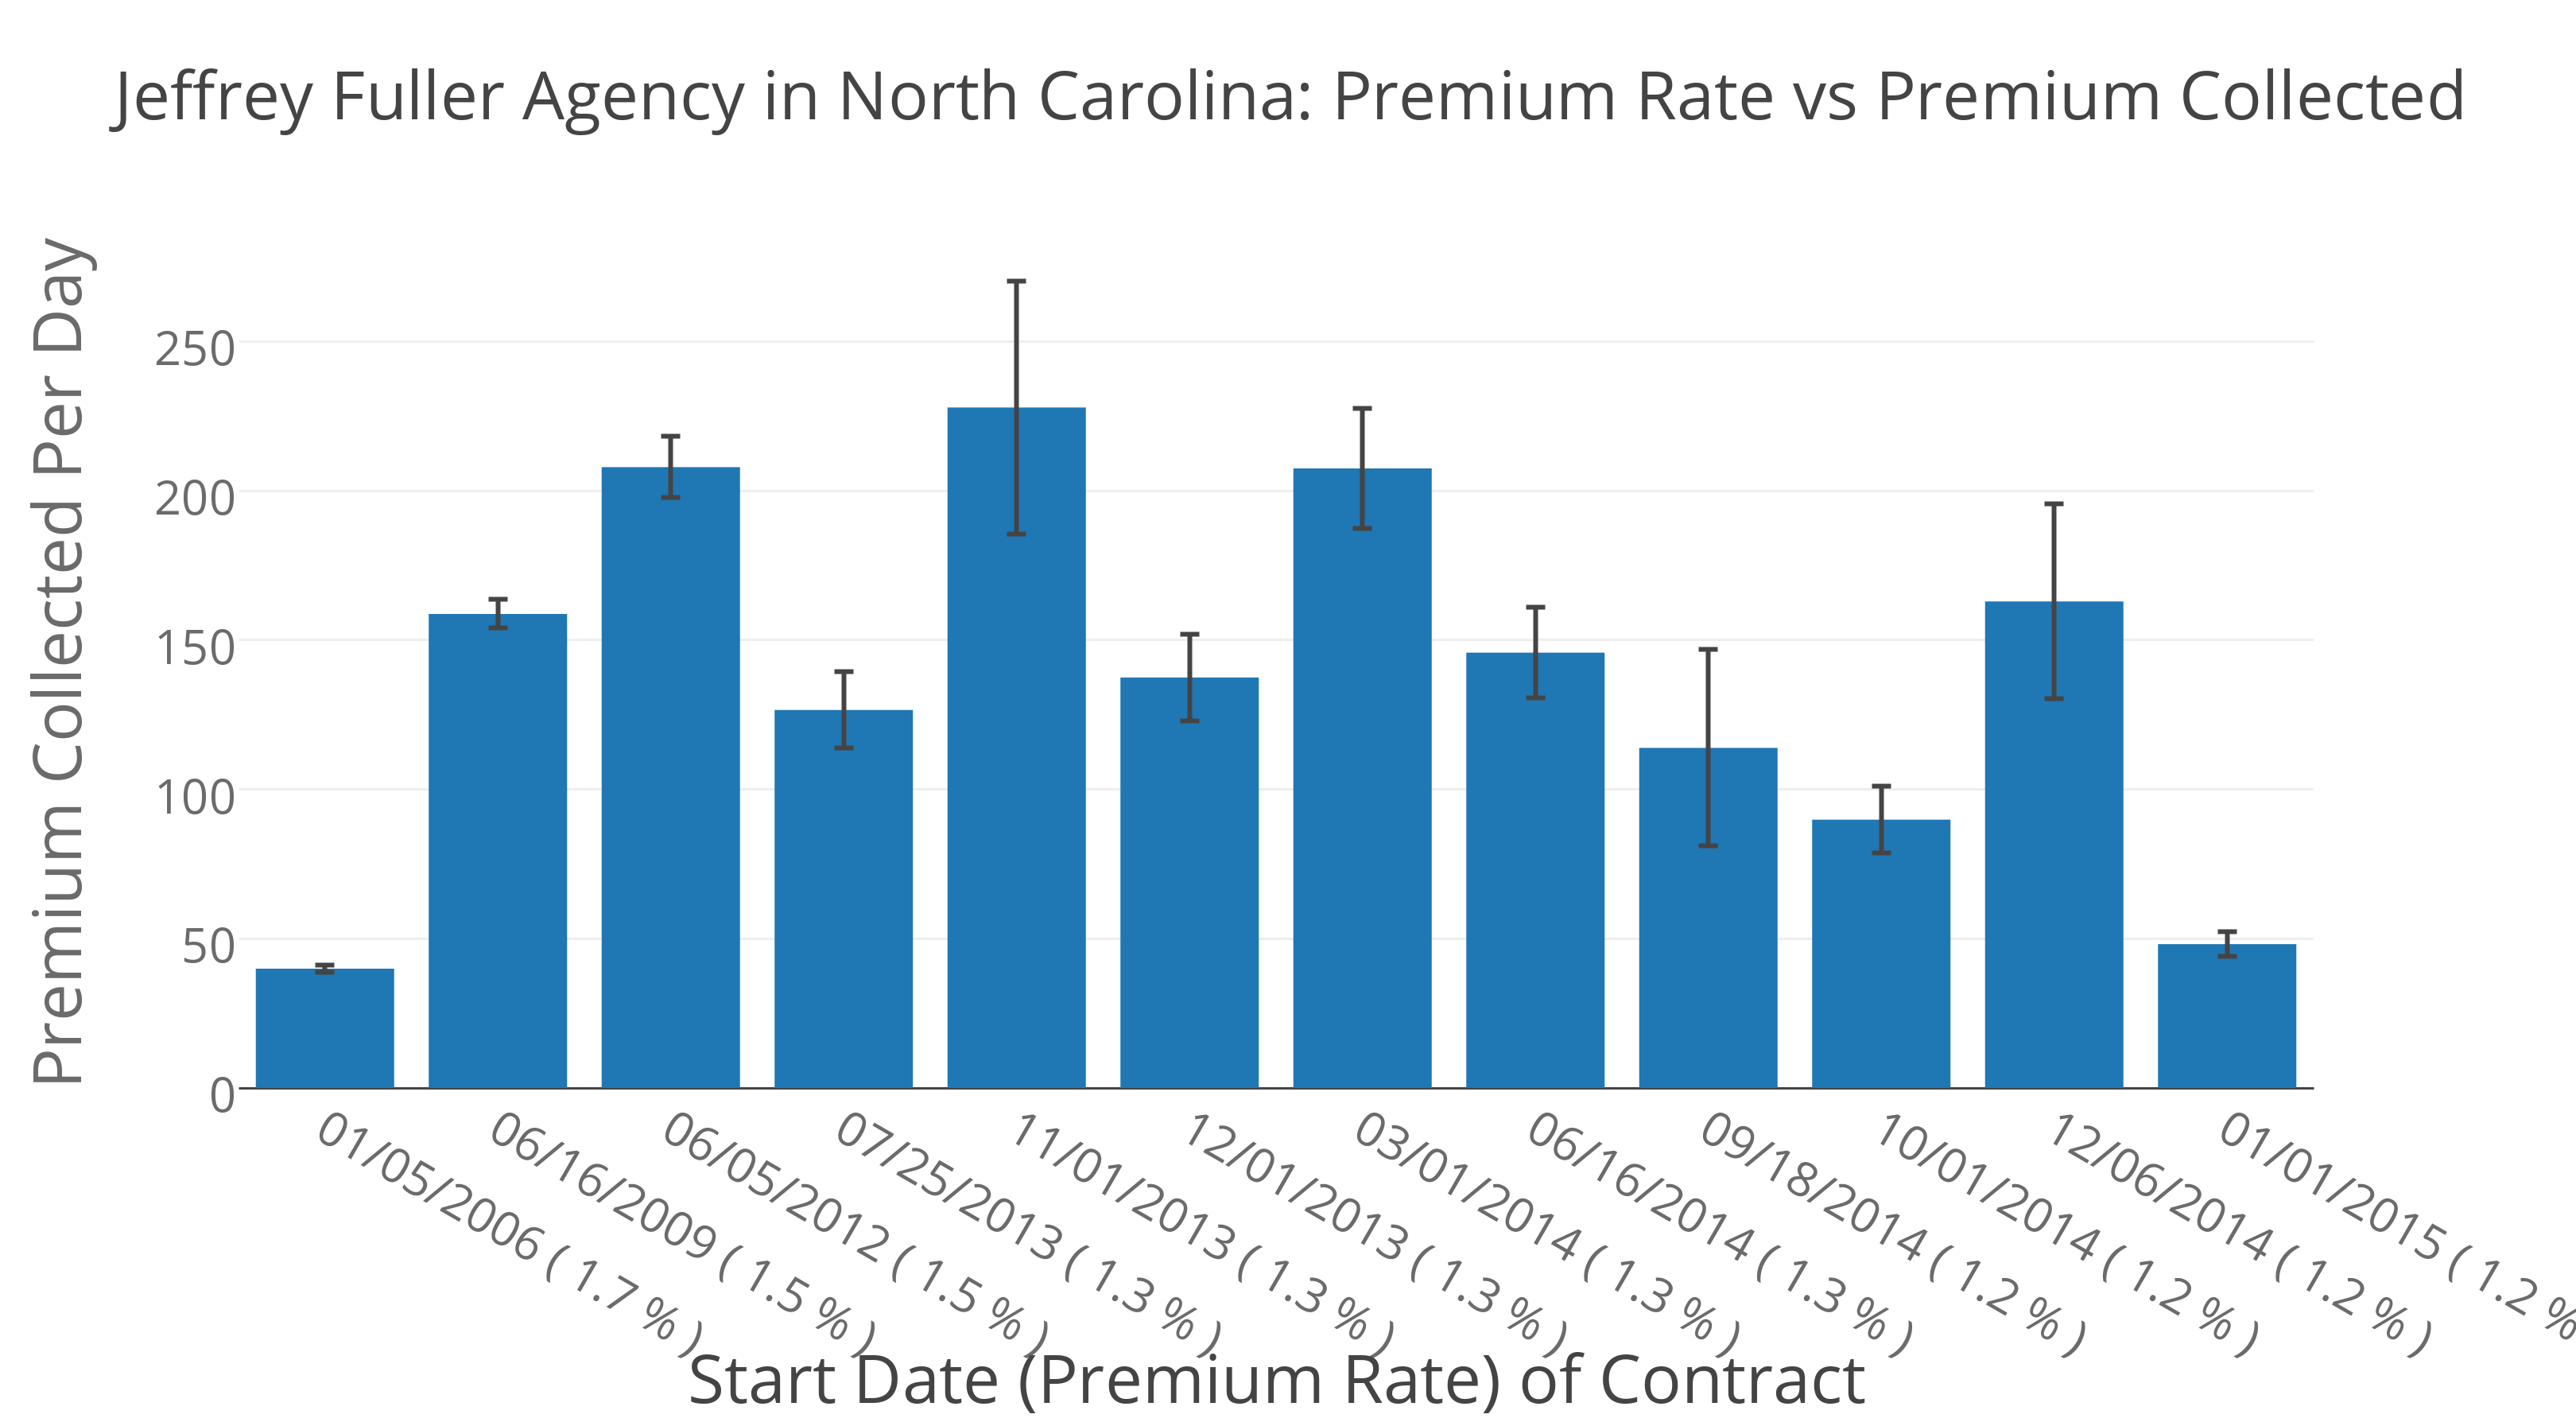
\includegraphics[width=\textwidth]{Jeffrey_Fuller_Agency_in_North_Carolina-_Premium_Rate_vs_Premium_Collected.png}
\end{subfigure}
\begin{subfigure}[b]{0.5\textwidth}
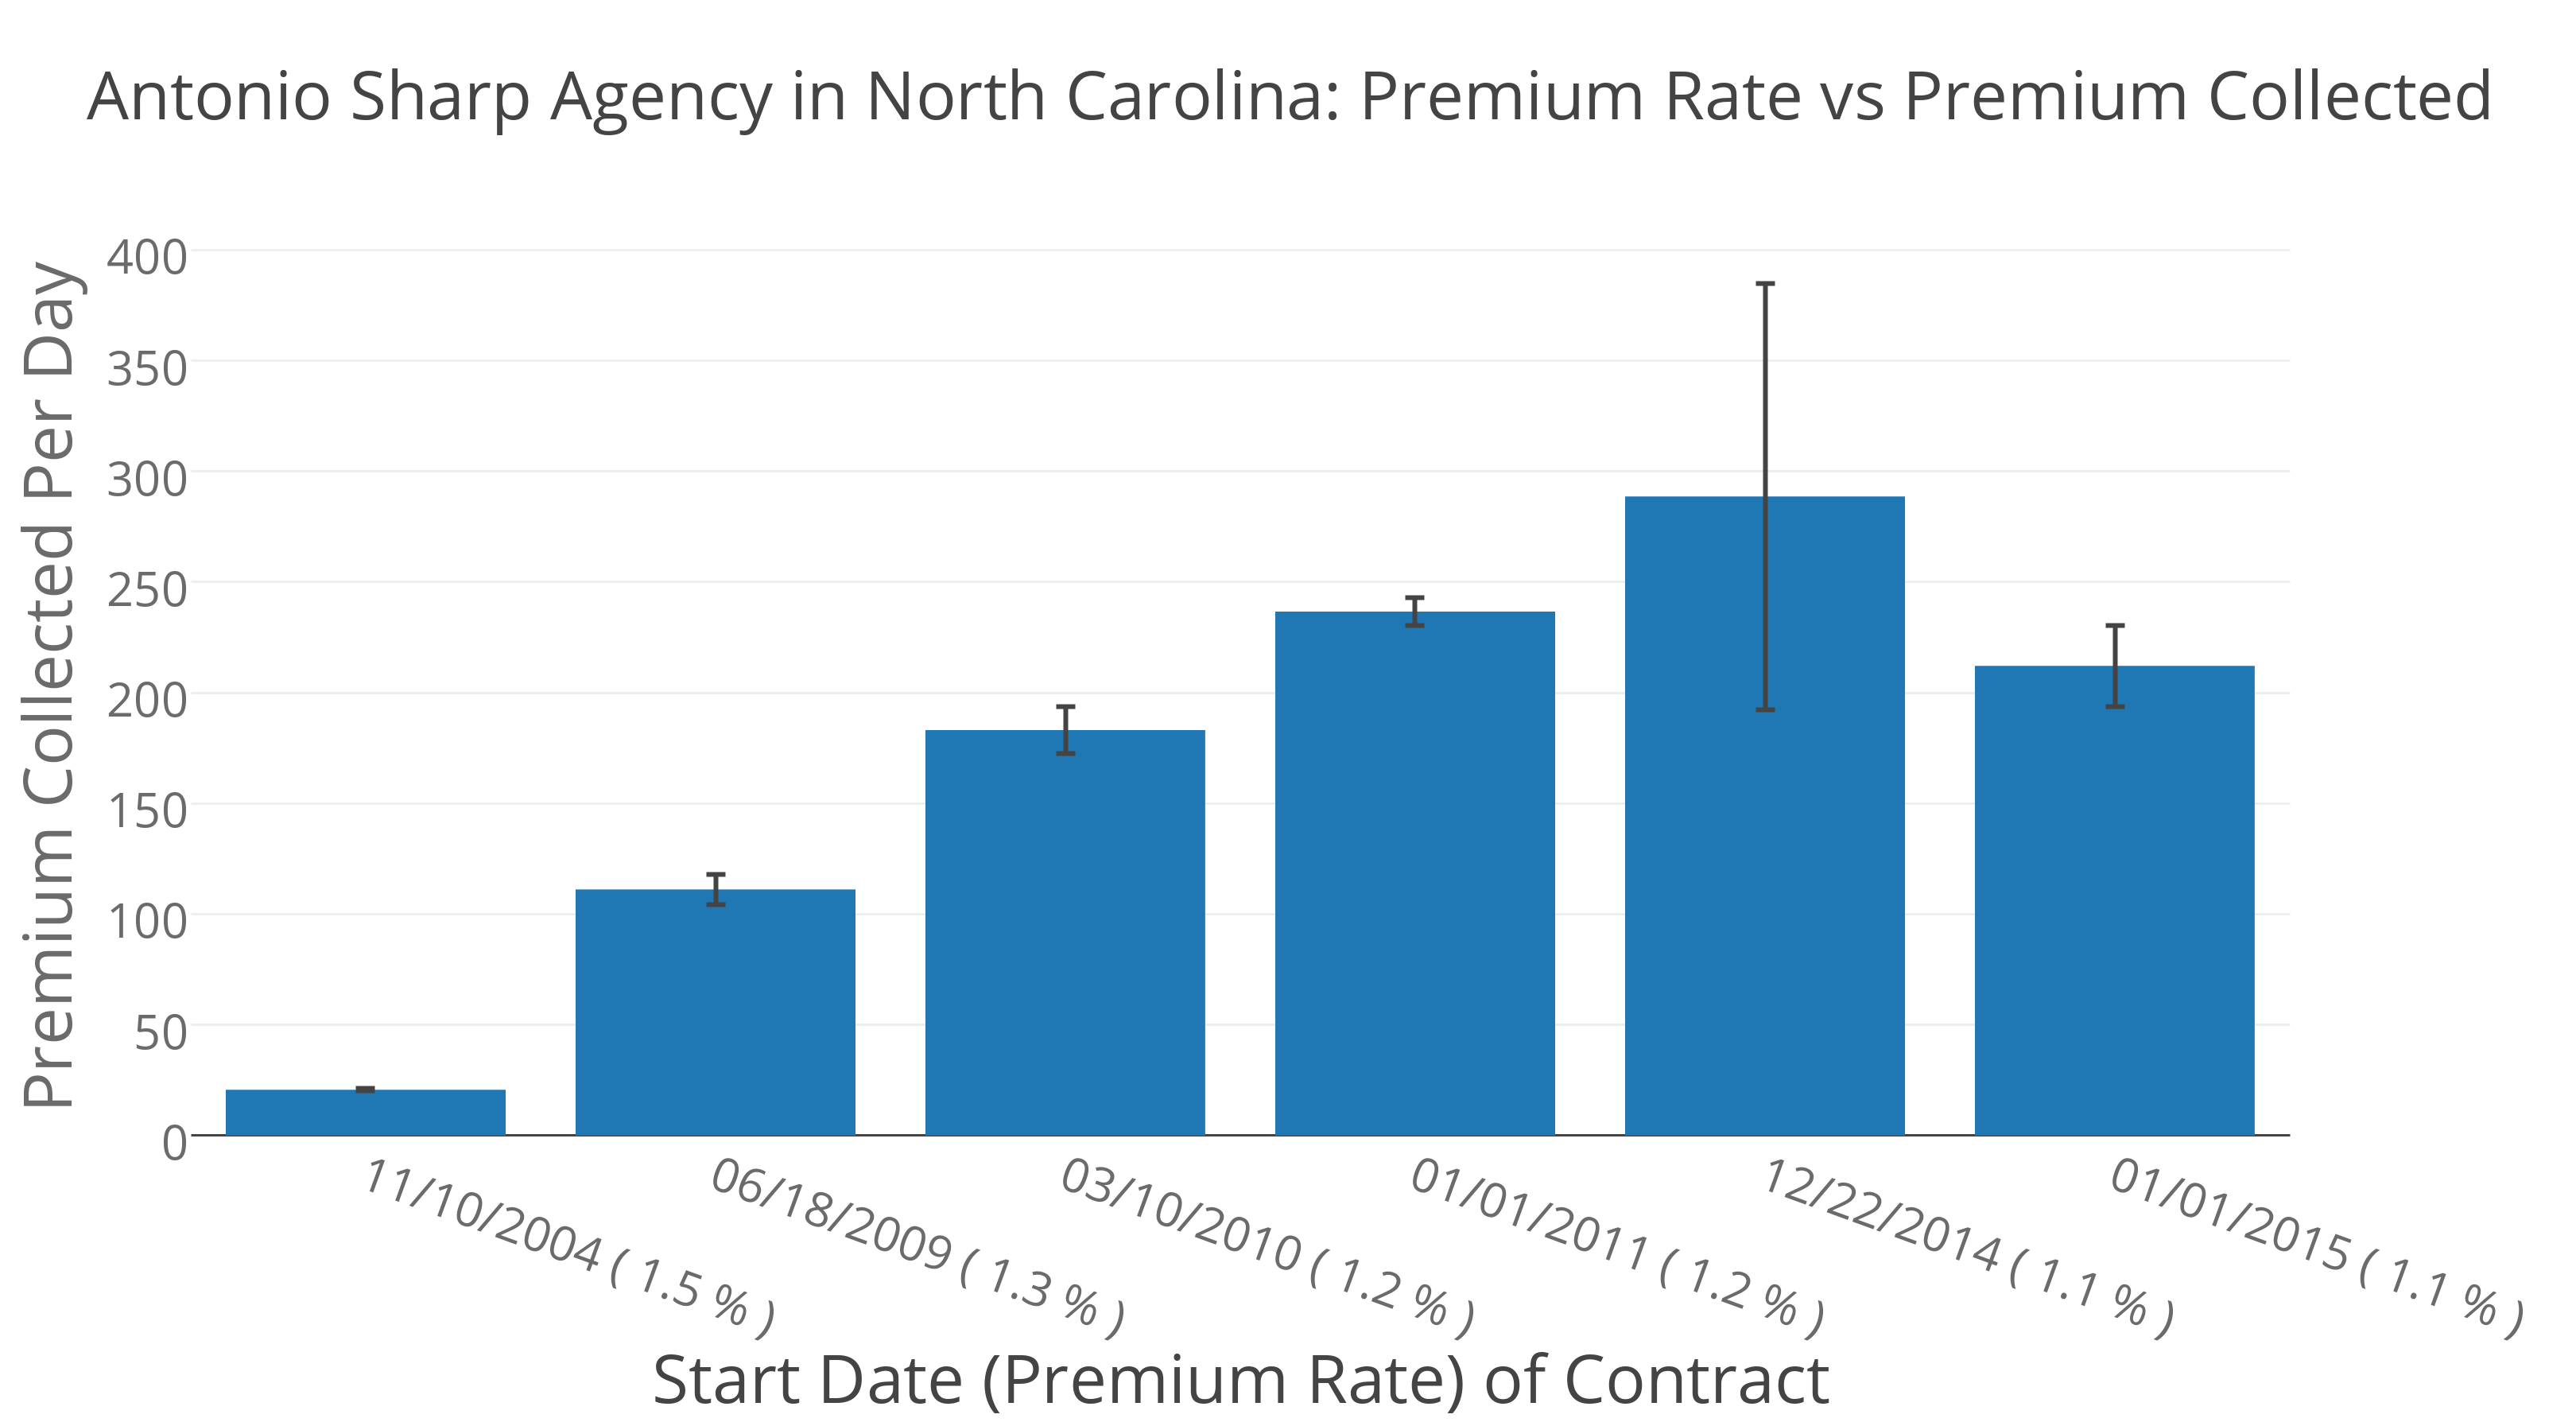
\includegraphics[width=\textwidth]{Antonio_Sharp_Agency_in_North_Carolina-_Premium_Rate_vs_Premium_Collected.png}
\end{subfigure}
\begin{subfigure}[b]{0.5\textwidth}
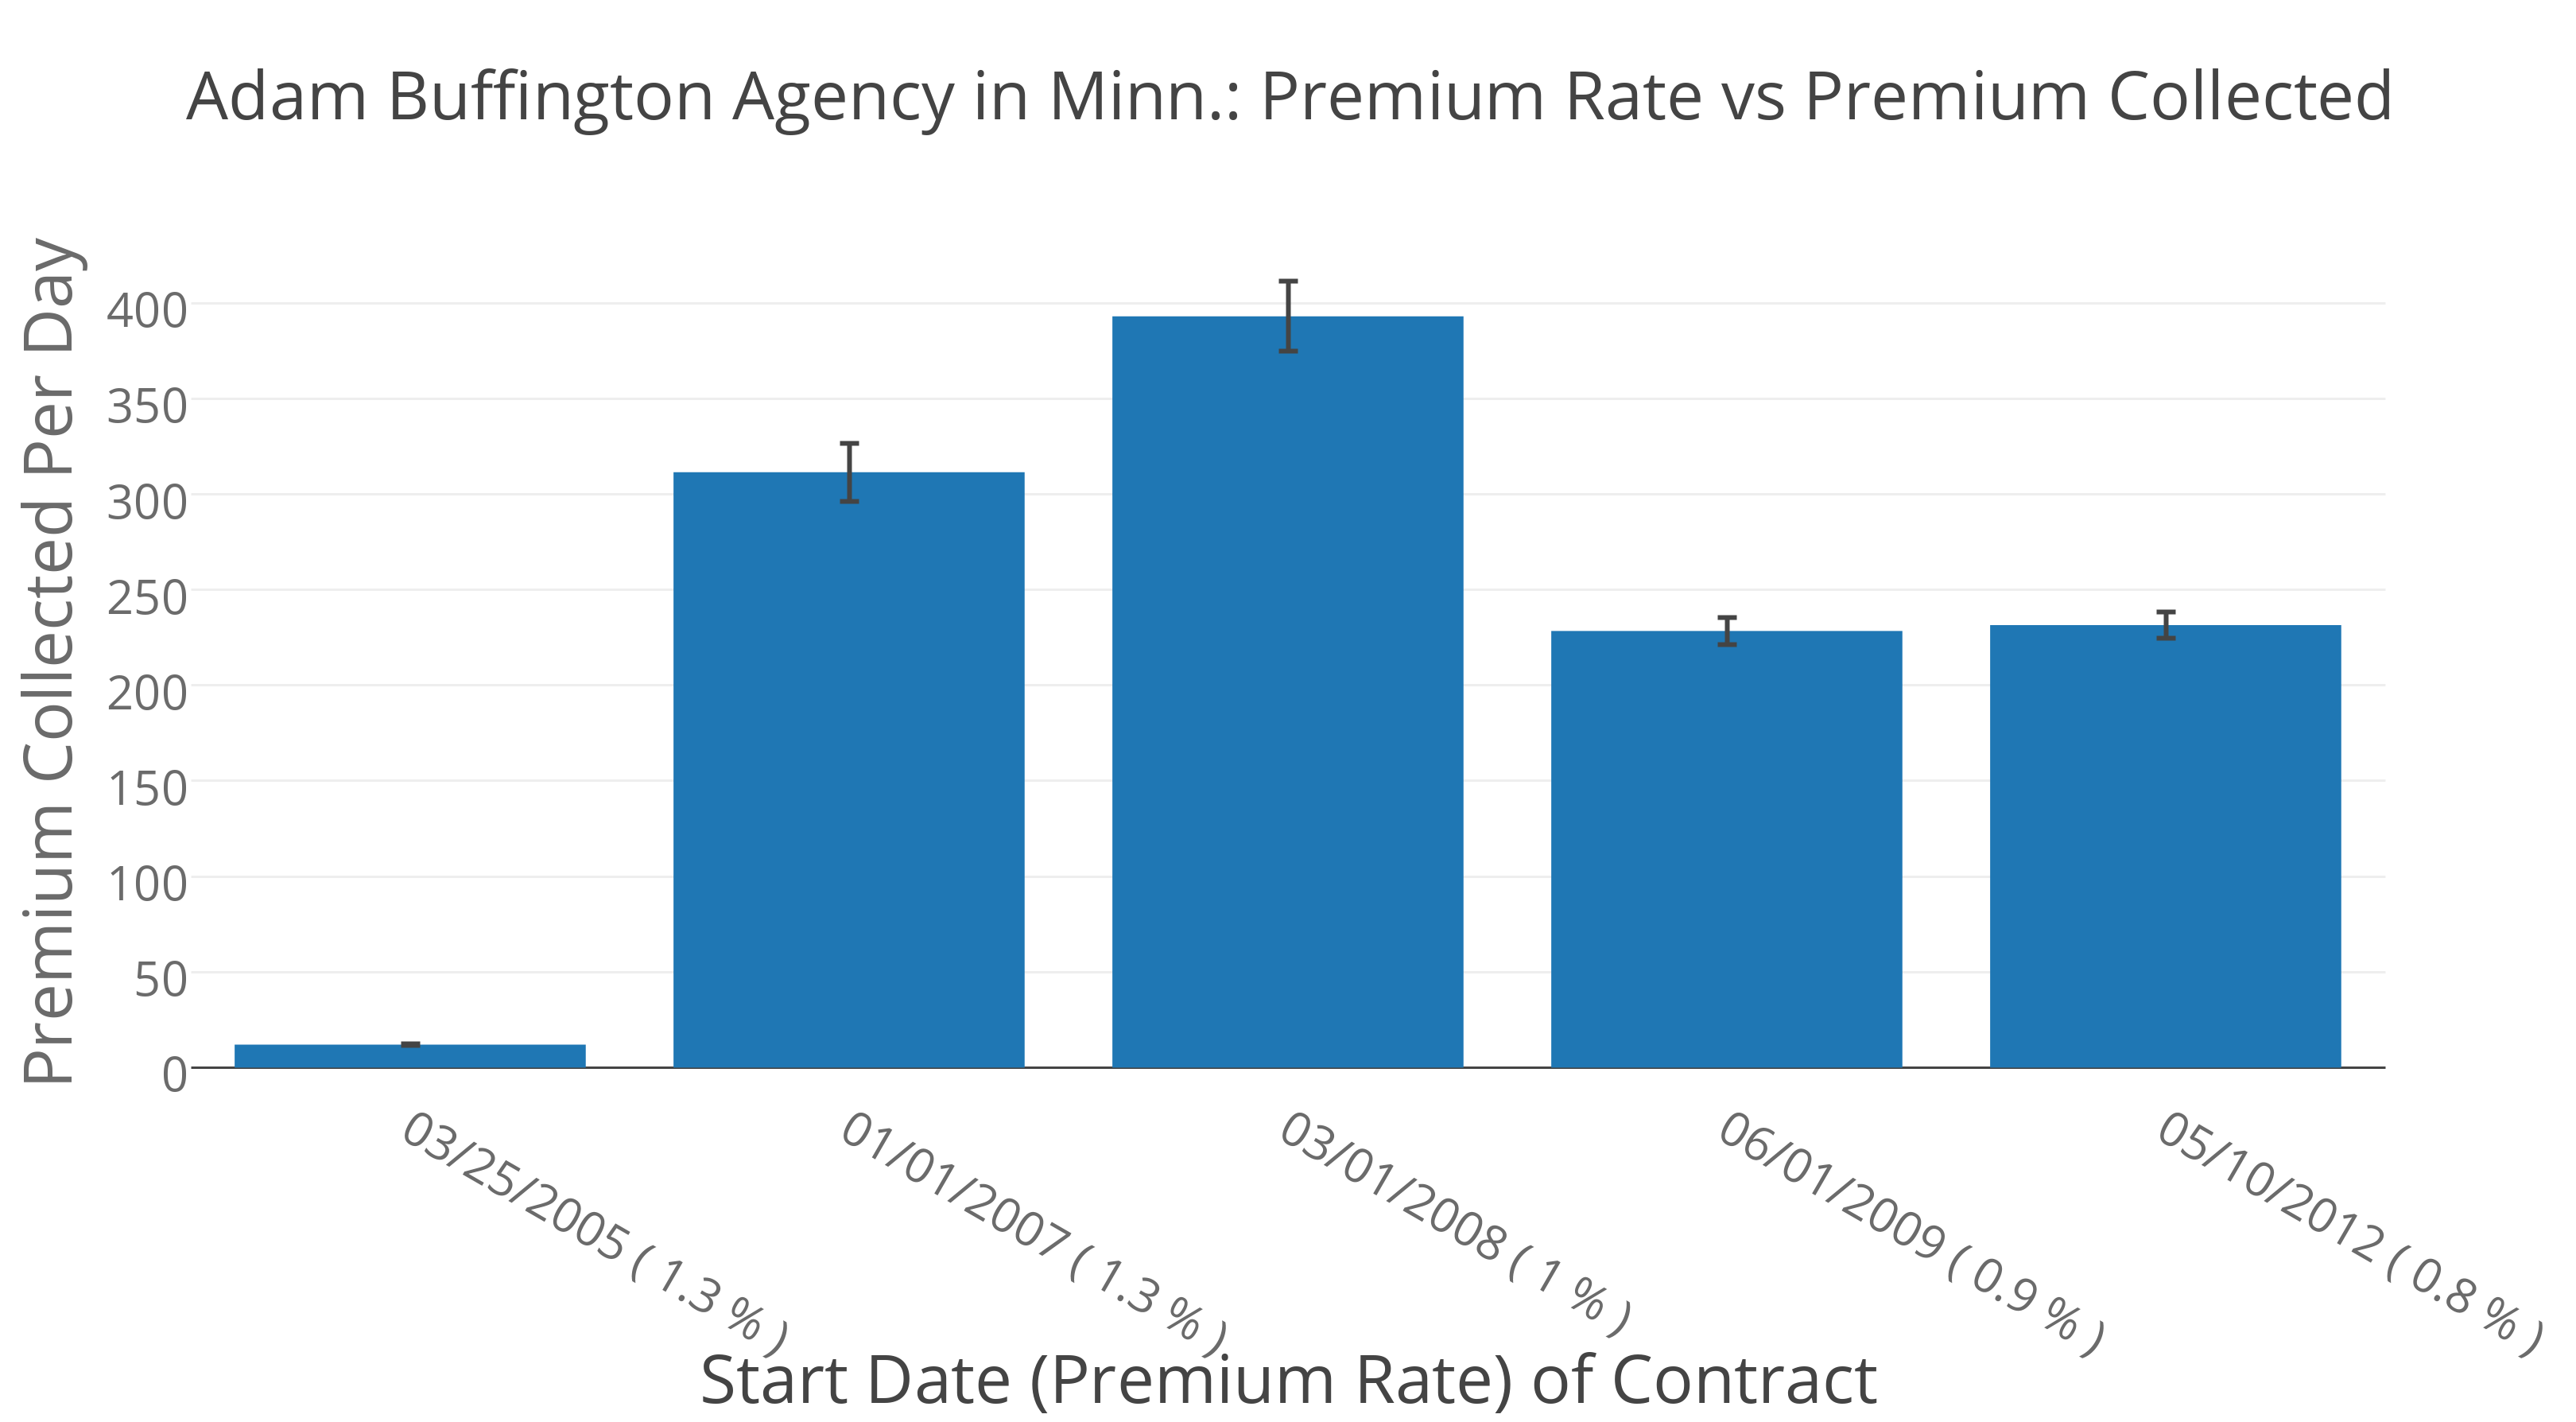
\includegraphics[width=\textwidth]{Adam_Buffington_Agency_in_Minn-_Premium_Rate_vs_Premium_Collected.png}
\end{subfigure}
\begin{subfigure}[b]{0.5\textwidth}
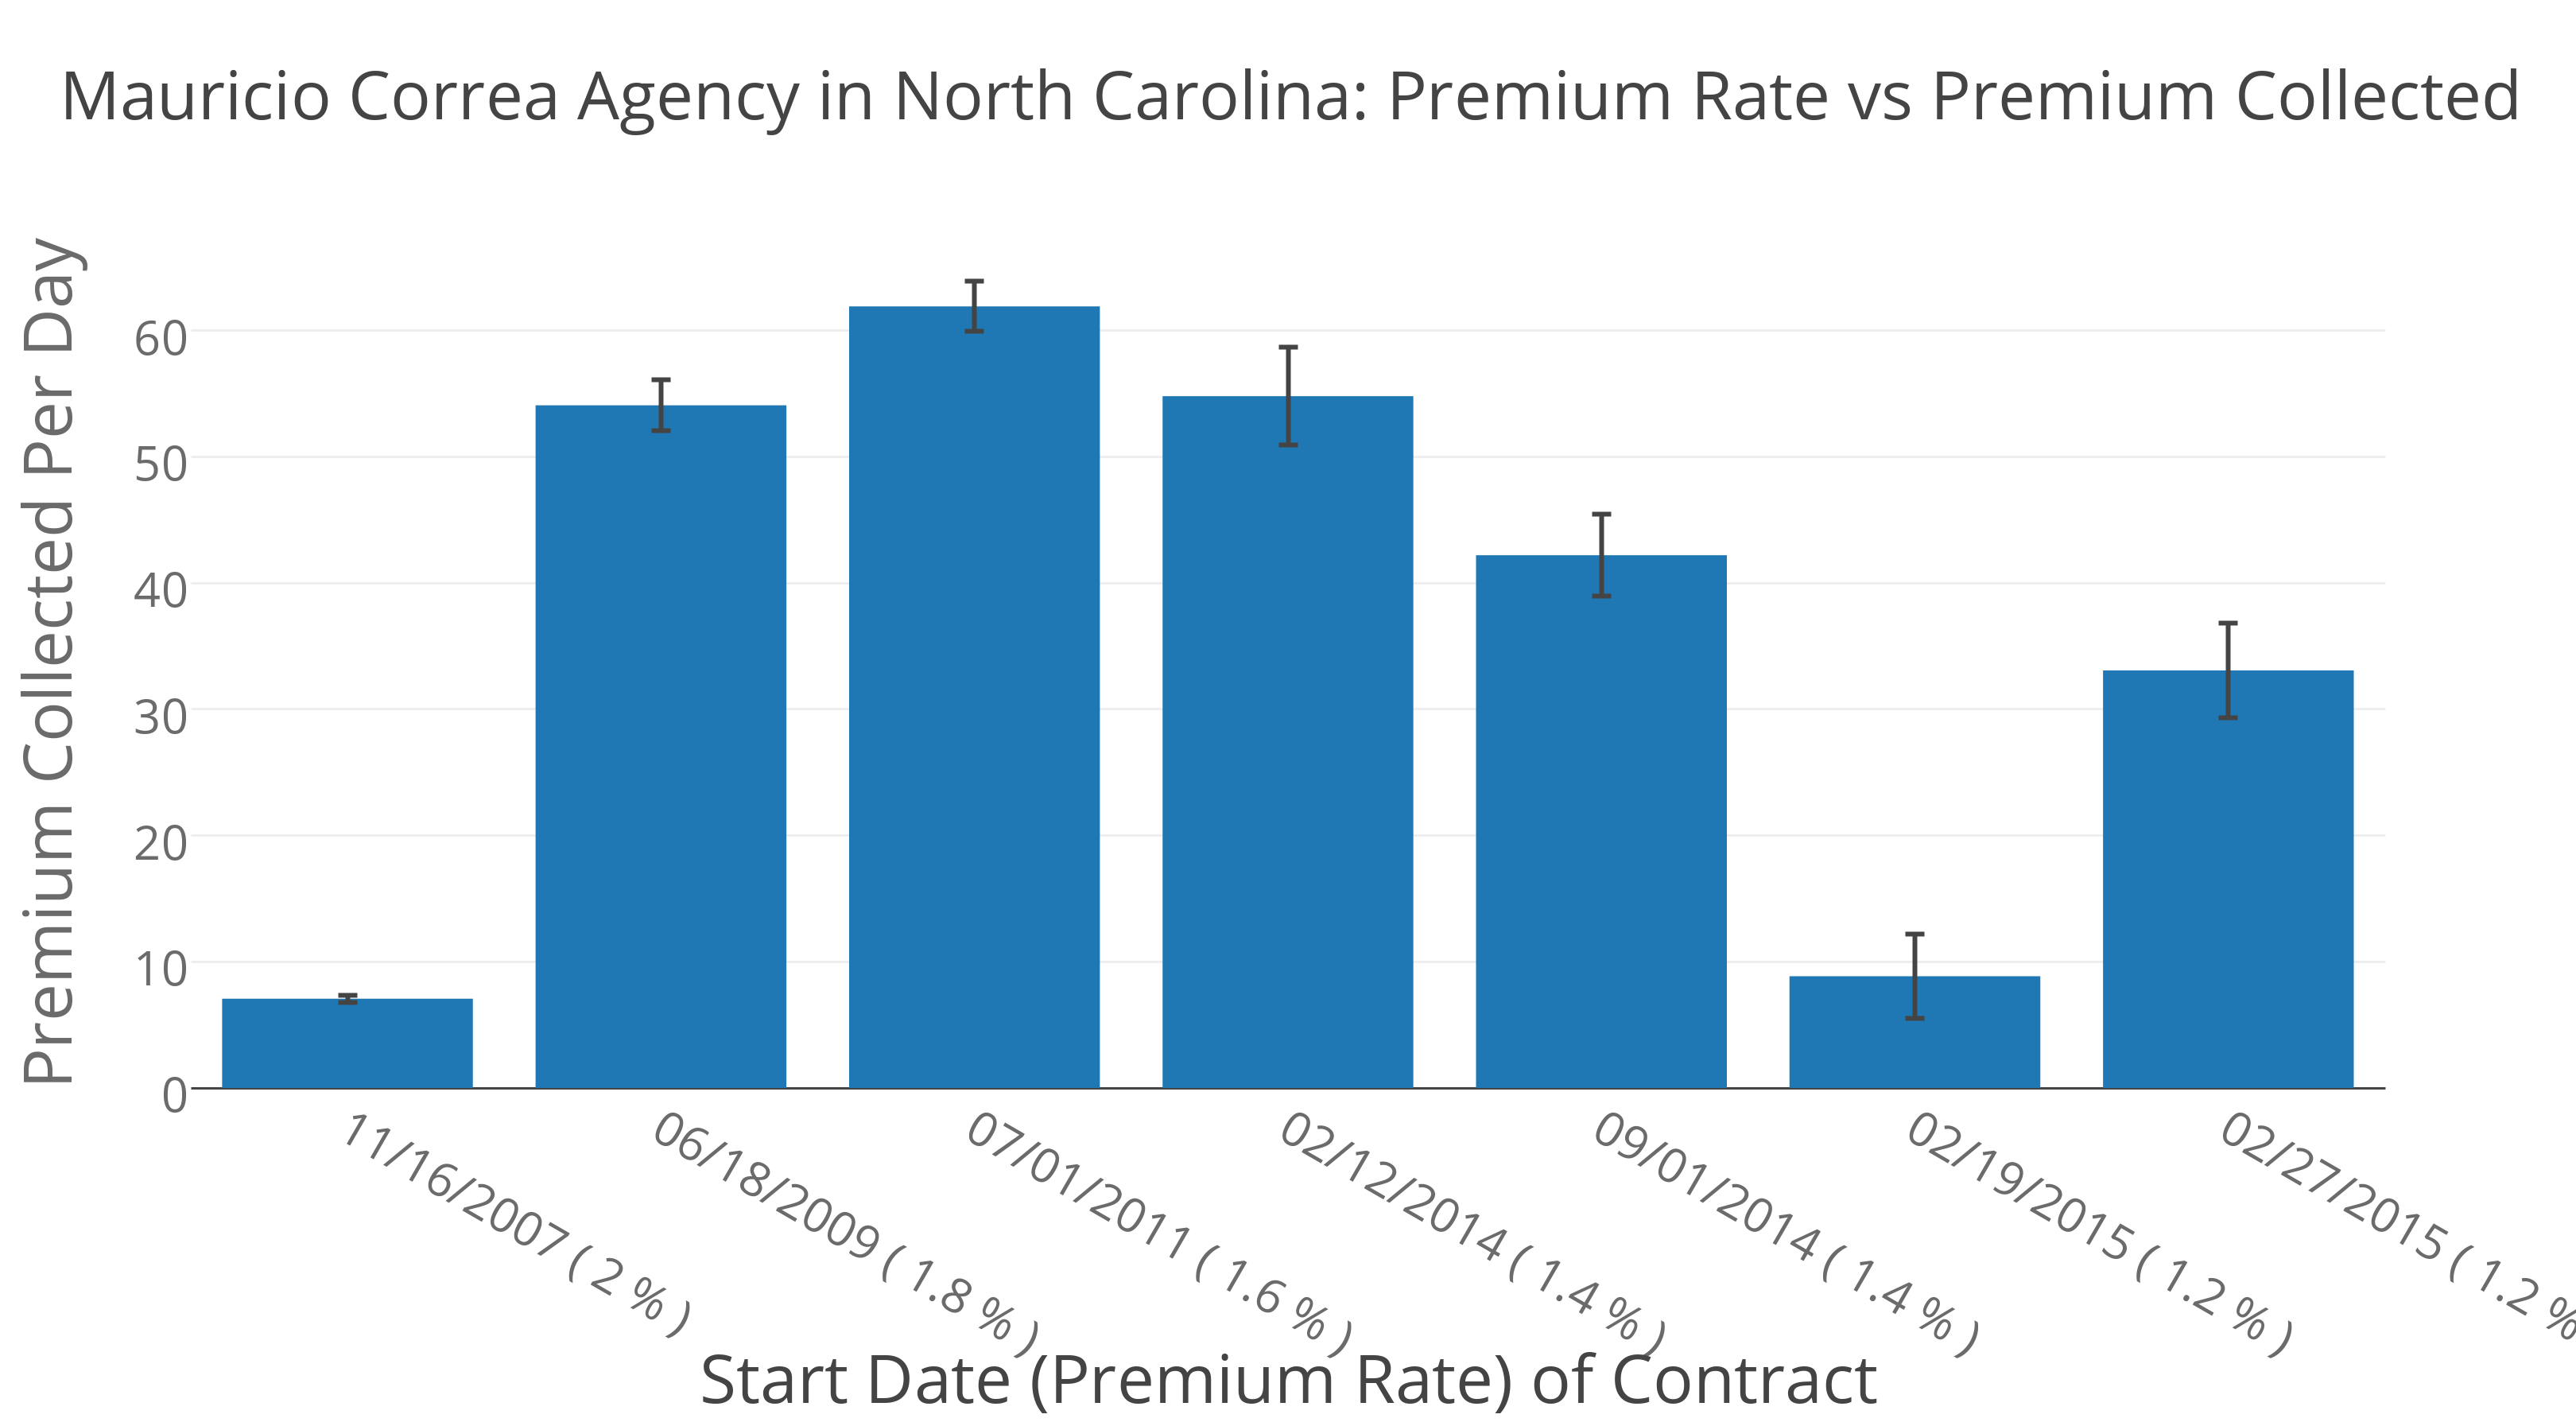
\includegraphics[width=\textwidth]{Mauricio_Correa_Agency_in_North_Carolina-_Premium_Rate_vs_Premium_Collected.png}
\end{subfigure}
\caption{Agents with varying premium rates}
\end{figure}
\end{center}
~\\
Looking at the different agencies, it becomes apparent that on average each write varying volume of penal per day.
A normalization is applied in order to be able to relate these agencies with one model.
~\\
~\\
As a start we plot the premium collected vs. the premium rate:

\begin{figure}[H]
\centering
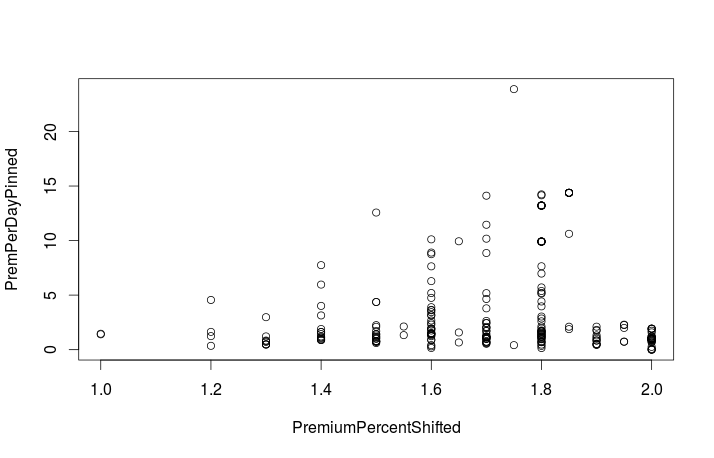
\includegraphics[width=0.45\paperwidth]{premPinnedNoLine.png}
\end{figure}
~\\
We can construct a linear model which relates the premium collected from agents as a function of premium rate.

\begin{figure}[H]
\centering
\begin{BVerbatim}
Residuals:
   Min     1Q Median     3Q    Max 
-4.875 -2.978 -1.478  1.250 19.538 

Coefficients:
                      Estimate Std. Error t value Pr(>|t|)    
(Intercept)             -6.677      2.694  -2.478  0.01406 *  
PremiumPercentShifted    6.299      1.613   3.905  0.00013 ***
---
Signif. codes:  0 ‘***’ 0.001 ‘**’ 0.01 ‘*’ 0.05 ‘.’ 0.1 ‘ ’ 1

Residual standard error: 4.266 on 197 degrees of freedom
Multiple R-squared:  0.07183,Adjusted R-squared:  0.06712 
F-statistic: 15.25 on 1 and 197 DF,  p-value: 0.0001296
\end{BVerbatim}
\end{figure}
~\\
The p-value for premium rate indicates that the variable is significant.  Meaning the 
model would perform much worse if the variable is taken out. But the adjusted R-squared value is
near 7\%, indicating that only a small amount of the variation in the data is explained by the current model.
~\\
~\\
This becomes more evident when we plot the fit on top of the data:

\begin{figure}[H]
\centering
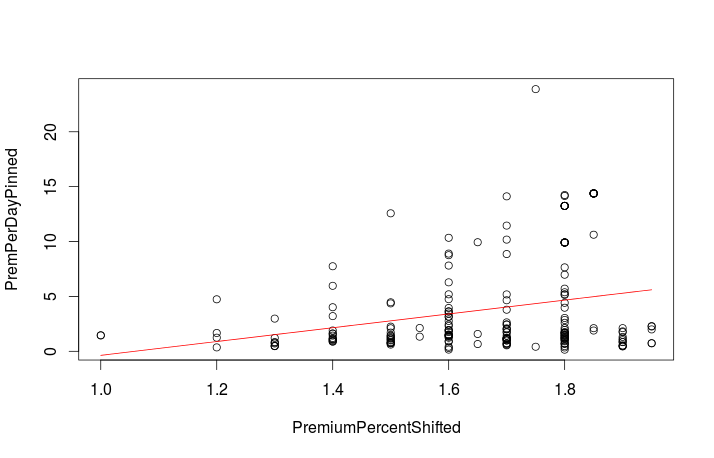
\includegraphics[width=0.45\paperwidth]{pinnedPremPerDay.png}
\end{figure}


Let's try to improve the model by adding another variable: The underwriting limit. \\

\begin{figure}[H]
\begin{center}
\begin{BVerbatim}
Residuals:
   Min     1Q Median     3Q    Max 
-5.875 -2.808 -1.090  1.548 20.339 

Coefficients:
                        Estimate Std. Error t value Pr(>|t|)    
(Intercept)           -4.885e+00  2.634e+00  -1.854   0.0652 .  
UnderWritingLimit      1.253e-05  3.118e-06   4.020  8.3e-05 ***
PremiumPercentShifted  4.102e+00  1.648e+00   2.489   0.0136 *  
---
Signif. codes:  0 ‘***’ 0.001 ‘**’ 0.01 ‘*’ 0.05 ‘.’ 0.1 ‘ ’ 1

Residual standard error: 4.111 on 196 degrees of freedom
Multiple R-squared:  0.1425,Adjusted R-squared:  0.1338 
F-statistic: 16.29 on 2 and 196 DF,  p-value: 2.856e-07
\end{BVerbatim}
\end{center}
\end{figure}
~\\
We see that the significance of the premium rate drops (but is still significant), while the underwriting limit 
plays an important role in the model.  The adjusted R-squared has doubled from our previous model, i.e. the model
does a better job of explaining the variations in the data.  We see this better below:

\begin{figure}[H]
\centering
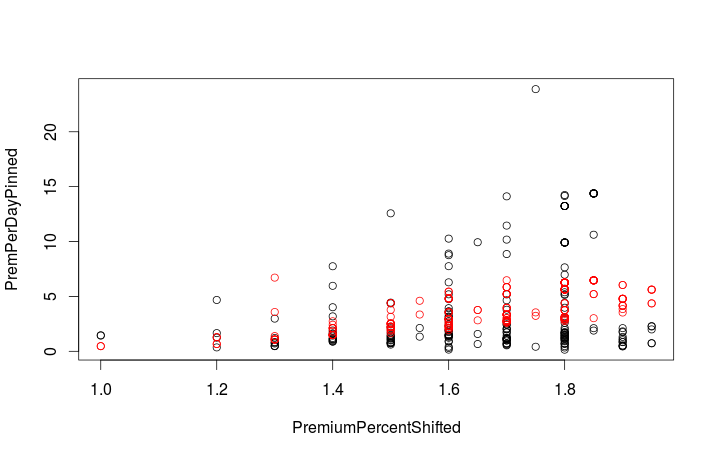
\includegraphics[width=0.45\paperwidth]{pinnedPremPerDayWithUWL.png}
\end{figure}

The aim is to continuously improve the model to increase the R-squared 
value by adding relevant variables. In some fields, it is entirely expected 
that your R-squared values will be low. For example, any field that attempts 
to predict human behavior, such as psychology, typically has R-squared values 
lower than 50\%. Humans are simply harder to predict than, say, physical processes.

\subsubsection{Deliverables and Work Estimate}
This project aims to build a ranking system which would allow to establish the health of agencies and in turn of AIA.
After the ranking is validated, a question underlying the ranking is formulated and answered through a detailed analysis. 
The exact question is to be determined after the ranking is established in order to ensure the correct and relevant question is asked.   
~\\
~\\
\textbf{1.5 month at \$80/hour = \$19,200}

\end{document}

